\documentclass[12pt,a4paper]{report}
%\usepackage[utf8]{inputenc}
\usepackage[spanish]{babel}
\usepackage{amsmath}
\usepackage{amsfonts}
\usepackage{amssymb}
\usepackage{booktabs}
\usepackage{subcaption}
\usepackage{caption}
\DeclareCaptionLabelFormat{tablename}{\textbf{Tabla #2}}
\DeclareCaptionLabelFormat{figurename}{\textit{#1 \thefigure}}
\captionsetup[figure]{labelformat=figurename}

%\captionsetup[table]{labelformat=tablename}
\captionsetup[table]{labelformat=tablename, labelsep=none, justification=raggedright, singlelinecheck=off}

\usepackage{verbatim}
\usepackage{graphicx}
\usepackage{animate}
\usepackage{float}
% \usepackage{cite}
\usepackage[left=2.75cm,right=2.6cm,top=3.5cm,bottom=3.5cm]{geometry}
\setlength{\parskip}{5pt}
  % Paquete para manejar citas numeradas
\usepackage{titletoc}
% Keywords command
\usepackage[spanish]{babel}
\usepackage{csquotes}
\usepackage[style=apa, backend=biber]{biblatex}

%\DeclareFieldFormat[thesis]{type}{(#1)}
\addbibresource{Bibliografia_TFT.bib}
\DefineBibliographyStrings{spanish}{ bibliography = {Referencias} }
\usepackage{array}

\providecommand{\keywords}[1]
{
  \small	
  \textbf{\textit{Palabras clave:\hspace{0.3cm}}} #1
}

%\bibliographystyle{unsrt}
\setlength{\bibitemsep}{1.25\baselineskip}

\usepackage[table]{xcolor}
\definecolor{naranja}{HTML}{E65113}
\usepackage[shortlabels]{enumitem}
\definecolor{slcolor}{HTML}{E65113}
\newcommand{\headlinecolor}{\color{slcolor}}
\usepackage{titlesec}

\definecolor{gray75}{gray}{0.75}
\newcommand{\hsp}{\hspace{-10pt}}

\usepackage{chngcntr}
\counterwithout{figure}{chapter}
\counterwithout{table}{chapter}

%%%%%%%%%%%%%%%%%%%%%%%%%%%%%%%%%%%%%%%%%%%%%%%%%%%%%%%%%%%%%%%%%%%%%%%%%%%%%
%------------------COMANDOS PARA EL TIPO DE LETRA---------------------------%
\usepackage{fontspec}
\usepackage[T1]{fontenc}
\usepackage{helvet}
\renewcommand{\familydefault}{\sfdefault}

\titleformat{\chapter}[hang]{\vspace{-3cm}\headlinecolor\Huge\bfseries}{\thechapter.\hsp}{20pt}{\Huge\bfseries}

%\titleformat{\section}[hang]{\Large\bfseries}{}{20pt}{\Large\bfseries}

\titleformat{\subsection}[hang]{\normalsize\bfseries}{}{20pt}{\large\bfseries}
\titleformat{\appendix}[hang]{\vspace{-3cm}\headlinecolor\Huge\bfseries}{\thechapter.\hsp}{20pt}{\Huge\bfseries}


%%%%%%%%%%%%%%%%%%%%%%%%%%%%%%%%%%%%%%%%%%%%%%%%%%%%%%%%%%%%%%%%%%%%%%%%%%%%%
%-------------------COMANDOS PARA TABLAS  E IMAGENES ---------------------%
\usepackage{tikz}
\usepackage{tabularx}
\renewcommand{\tablename}{Tabla}
%%%%%%%%%%%%%%%%%%%%%%%%%%%%%%%%%%%%%%%%%%%%%%%%%%%%%%%%%%%%%%%%%%%%%%%%%%%%%
%----------------- COMANDOS PARA CABECERAS Y PIE DE PAGINA -----------------%
\usepackage{lastpage}
\usepackage{fancyhdr}
\usepackage{tikz}  % Necesario si quieres usar imágenes con TikZ, aunque no se usará en este caso

\fancypagestyle{plain}{%
  \renewcommand{\headrulewidth}{0pt}  % Eliminar la línea del encabezado
  \fancyhead{}  % Eliminar cualquier contenido en el encabezado
  \fancyfoot{}  % Eliminar cualquier contenido en el pie de página
  \fancyfoot[C]{\thepage}  % Mostrar solo el número de página en el centro del pie de página
}

\pagestyle{plain}  % Aplicar este estilo en el documento




%%%%%%-------------------+++++++++--INICIO DEL DOCUMENTO--+++++++++---------------------------%%%%%

\begin{document}



%------------------XXXX++++++ INICIO DE PORTADA  ++++++XXXXX-----------------%
\begin{titlepage}

\newgeometry{left=2.5cm, bottom=3cm, top=2cm, right=2.5cm}

\tikz[remember picture,overlay] \node[opacity=1,inner sep=0pt] at (73.6mm, -124.25mm){
\includegraphics{./Images/Picture_TitlePage.jpg}};

{\fontfamily{phv}\selectfont
\fontsize{22}{10.4}\fontseries{b}\selectfont
\vspace{14cm}
\textbf{Predicción de la demanda de energía eléctrica mediante modelos de
Machine Learning}

\bigskip

\fontsize{12}{12}\selectfont
\fontseries{m}\selectfont
\vspace{5cm}
\centering
\begin{tabularx}{1\textwidth} { 
  || >{\raggedright}X 
  || >{\centering}X 
  || >{\raggedleft\arraybackslash}X || }
 Titulación:\\Máster en Big Data y Ciencia de datos\\ 
 & Alumno/a: Valverde Navarro, Gregorio\\DNI: 23827388D
 & Convocatoria: \\
 Curso Académico\\ 2023-2024 
  & Director/a del TFT: Álvarez Torres, Pedro   
  & SEGUNDA  \\
\end{tabularx}
 }
\end{titlepage}
%--------------------XXXX++++++ FIN DE PORTADA  ++++++XXXXX-----------------%

\thispagestyle{empty}
\mbox{}
\newpage

\pagenumbering{roman}

%\addcontentsline{toc}{chapter}{Índice general}
\tableofcontents	

\clearpage
\mbox{}
\thispagestyle{empty}
\newpage

%\addcontentsline{toc}{chapter}{\listfigurename}
\renewcommand{\listtablename}{Índice de tablas}
\listoffigures

\clearpage
\mbox{}
\thispagestyle{empty}
\newpage

%\addcontentsline{toc}{chapter}{\listtablename}
\listoftables

\clearpage
\mbox{}
\thispagestyle{empty}
\newpage

\chapter*{Agradecimientos} 
%\addcontentsline{toc}{chapter}{Agradecimientos} 

En primer lugar, me gustaría agradecer a mi tutor, D. Pedro Álvarez Torres, la gran confianza que ha depositado en mí. Sus ánimos, incluso en los momentos difíciles fuera de lo académico, así como sus consejos y directrices claras, han sido una guía invaluable a lo largo del desarrollo del proyecto.

No puedo dejar de mencionar primero a mi mejor amigo, Juan, quien siempre ha estado ahí para apoyarme y ayudarme en todos los aspectos de mi vida. 

Quiero agradecer también a mi familia: a mi madre, por esa fuerza tan inspiradora; a mi padre, por la calma y la firmeza de sus palabras; y, como no, a mi hermana Gloria, por recordarme que la vida no es solo cálculos y que vale la pena cultivar una vena creativa. No puedo olvidar a mis abuelos, tíos y primos, especialmente a mi abuela Juana, con quien he tenido la suerte de crecer y compartir innumerables lecciones que llevaré conmigo siempre. 

Además, quiero agradecer a Elena, esa persona que, aunque ha llegado recientemente a mi vida, me ha demostrado que el tiempo no es más que un simple número. 

Sin vosotros no habría sido capaz de encontrar mi vocación, esto no es más que el inicio. Gracias a todos.

\clearpage
\mbox{}
\thispagestyle{empty}
\newpage

\chapter*{Resumen} 
%\addcontentsline{toc}{chapter}{Resumen} 

El mercado eléctrico constituye una de las bases de la economía más relevantes en la actualidad, generando movimientos millonarios de capital cada día. La infraestructura industrial y tecnológica depende de la electricidad, un bien de consumo que enfrenta múltiples desafíos, siendo uno de los principales la dificultad para su almacenamiento. Esto requiere la implementación de técnicas que satisfagan las necesidades de la población, incluso durante picos de alta demanda.

Paralelamente, el mundo de los datos avanza a pasos agigantados. El crecimiento exponencial de la información impulsa el desarrollo de campos como la inteligencia artificial y el Big Data, lo que genera una necesidad creciente de aplicar estas tecnologías para gestionar la demanda eléctrica. Actualmente, se emplean diversas técnicas de predicción para manejar los picos de consumo y evitar pérdidas económicas significativas. Entre ellas destacan el Machine Learning, las redes neuronales y técnicas tradicionales que utilizan estadística avanzada.

Comprender el contexto del proyecto es uno de los desafíos más importantes. Es fundamental poner especial énfasis en la elección de las variables a considerar, dado que se trata de un problema de alta complejidad. La demanda eléctrica depende de un amplio conjunto de factores externos, conocidos como variables exógenas, que influyen directamente en esta magnitud. Además, la etapa de extracción y preprocesamiento de datos es crucial, ya que la calidad de los datos disponibles puede mejorar o deteriorar significativamente los resultados.

Este estudio tiene como objetivo analizar el potencial de los algoritmos de Machine Learning en la predicción de la demanda eléctrica en comparación con otras técnicas. Se hará especial énfasis en el estudio de las variables que más influyen en la calidad de los resultados. Para ello, se definirán una serie de condiciones iniciales que permitirán realizar una comparación exhaustiva entre diferentes metodologías y extraer conclusiones valiosas. Aunque el propósito no es alcanzar el mejor resultado idílico de predicción, se busca determinar qué tipos de técnicas funcionan mejor en estos contextos. Se anticipa que las técnicas de Machine Learning ofrecerán resultados satisfactorios, aunque no necesariamente superiores a los de redes neuronales simples.

\


\vspace{0.5cm}

\keywords{machine, deep, learning, energy, demand}


\clearpage
\mbox{}
\thispagestyle{empty}
\newpage


\chapter{Introducción}\label{cap:cap1}

\pagenumbering{arabic}

Desde su descubrimiento e implementación, la electricidad ha generado una serie de necesidades esenciales en la sociedad. Como uno de los principales motores del desarrollo tecnológico, la electricidad está presente en nuestro día a día, tanto en actividades cotidianas como en la industria. Este recurso es considerado un pilar fundamental del desarrollo económico, y su creciente consumo, junto con las limitaciones en su almacenamiento, hace necesaria una mejora en el control de su demanda.

Redeia, o mejor conocida como la Red Eléctrica de España, es el operador del sistema eléctrico que establece las previsiones de la demanda de energía eléctrica del país. Además, se encarga de la transmisión de electricidad (\cite{Wikipedia2024}). Su trabajo más importante es la planificación eléctrica para conseguir un país más ecológico, que luche contra la emergencia climática mediante la integración de energías renovables, sin perder de vista la búsqueda del desarrollo económico y social del país. También busca un país más conectado, permitiendo abastecer las necesidades básicas de la sociedad (\cite{ree2024}).

Actualmente, existen diversas técnicas para predecir el consumo eléctrico, logrando márgenes de error cada vez más reducidos con el paso del tiempo. Las técnicas de inteligencia artificial se han convertido en las principales protagonistas en este ámbito. Aunque los algoritmos y métodos son fundamentales en la predicción de la demanda eléctrica, hay otro aspecto de gran relevancia: la selección de factores determinantes que influyen en dicha demanda. Estos factores, conocidos como variables exógenas, son elementos externos que afectan el consumo, pero que no están directamente controlados por el sistema eléctrico. Las principales variables pueden clasificarse en temporales, meteorológicas y económicas.

El desarrollo del proyecto sigue una estructura similar a la de un trabajo convencional de ciencia de datos: extracción, preprocesamiento, análisis exploratorio de los datos y entrenamiento de modelos. Los resultados se comparan y analizan con el fin de extraer conclusiones que aporten valor. En primer lugar, se lleva a cabo una investigación y un estudio de la bibliografía vigente, lo cual es crucial para tener un buen entendimiento del sector eléctrico. Esto abarca temas de cultura general, comprensión de su estructura y los factores que influyen en la demanda. Además, se realiza un análisis de los principales algoritmos utilizados en este ámbito, centrándose principalmente en Machine Learning, pero también incluyendo técnicas más convencionales y métodos avanzados como las series temporales y el Deep Learning. Tras este estudio general, se procede a la selección de las variables exógenas y de los modelos que se utilizan en el análisis.

A lo largo del desarrollo del trabajo, tanto en la redacción de la memoria como en la creación del código, se ha utilizado la herramienta de inteligencia artificial generativa ChatGPT (\cite{chatgpt}). Principalmente, se ha empleado para corregir errores ortográficos, mejorar la fluidez y estructura del texto de la memoria, y detectar errores básicos en el código, facilitando su corrección. Además, ha sido de gran utilidad para generar código en \LaTeX, especialmente en la creación de tablas, el mantenimiento de formatos, el uso de citas, entre otros. En general, ha resultado ser una herramienta eficaz que ha permitido ahorrar una gran cantidad de tiempo en tareas sencillas y ha servido de apoyo en la comprensión de conceptos básicos.

\section{Objetivos}

El proyecto está compuesto por una serie de objetivos previamente definidos que deben cumplirse a lo largo de su desarrollo. Su finalidad es establecer metas que orienten el camino a seguir. Estos objetivos se pueden clasificar en principales y secundarios.

\subsection{Objetivos principales}

El primer objetivo principal del proyecto es estudiar el potencial real de los algoritmos de Machine Learning en la predicción de la demanda eléctrica, comparándolos con otros algoritmos de características diferentes. El segundo objetivo se centra en analizar la influencia de las variables exógenas en los resultados, evaluando tanto sus relaciones fuertes como débiles con la variable objetivo.

\subsection{Objetivos secundarios}

Los objetivos secundarios están estrechamente relacionados con metas técnicas, fundamentadas en la aplicación de conocimientos adquiridos tanto en el máster como en fuentes externas.

En primer lugar, se busca realizar un estudio previo de los recursos disponibles para adquirir la formación y las habilidades necesarias que permitan cumplir los objetivos generales. Estos objetivos secundarios se basan en:

\begin{itemize}
    \item Proceso de estudio sistemático de diferentes recursos externos: artículos, webs, blogs, entre otros.

    \item Elección adecuada de los datos a trabajar y de los modelos a entrenar. Toma de decisiones adecuada. 
\end{itemize}

En cuanto a objetivos secundarios más técnicos:

\begin{itemize}
\item Preprocesamiento adecuado de los datos, garantizando fiabilidad, coherencia e integridad.

\item Análisis exploratorio de los datos enfocado a la transmisión de ideas o argumentos que apoyen el desarrollo del proyecto.

\item Entendimiento teórico profundo de los modelos.

\item Uso de técnicas adecuadas de optimización de hiperparámetros para garantizar los mejores resultados en el entrenamiento de los modelos.
\end{itemize}

Finalmente, también hay que tener en cuenta etapa final del proyecto:

\begin{itemize}
    \item Entendimiento del contexto de los datos y de los modelos utilizados. Asegurar una comprensión profunda del entorno en el que se desarrollan los datos y los modelos aplicados.

    \item Extracción de conclusiones orientadas a garantizar los objetivos generales propuestos.
\end{itemize}

\section{Planificación}

Para lograr los objetivos de manera satisfactoria, es fundamental llevar a cabo una planificación previa de la metodología a seguir, estableciendo intervalos de tiempo estimados. Con este fin, se ha elaborado un gráfico de tareas que abarca un período de tres meses, organizando las actividades en intervalos semanales, lo que equivale a un total de doce semanas.

\begin{figure}[H]
    \centering
    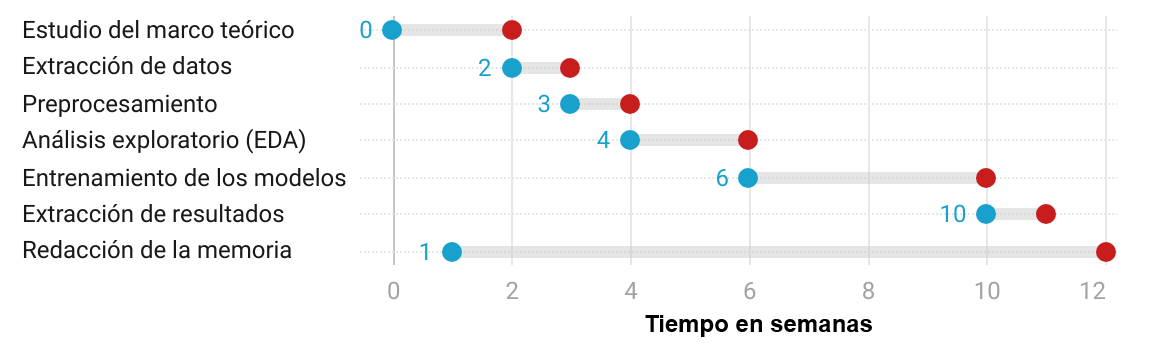
\includegraphics[width=1\textwidth]{Images/tfm-1.1.png}
    \caption{Cronograma inicial de tareas en intervalos semanales (Elaboración propia)}
    \label{fig:cronograma}
\end{figure}

La Figura \ref{fig:cronograma} muestra el cronograma inicial de tareas planteado para el desarrollo del proyecto. La elección de cada intervalo se basa en la experiencia adquirida en otros proyectos durante el máster, dividiéndose las tareas en:

\begin{itemize}
    \item \textbf{Estudio del marco teórico}: dos primeras semanas. Estudio de los fundamentos teóricos y de la bibliografía actualizada. Selección de artículos, blogs y otras fuentes.

    \item \textbf{Extracción de datos}: semana 2 a 3. Creación del programa para la extracción de los datos de las fuentes necesarias. Obtención de claves API necesarias.

    \item \textbf{Preprocesamiento}: semana 3 a 4. Código destinado al preprocesamiento de datos: unificación de datasets, adición de variables exógenas y tratamiento general de datos.

    \item \textbf{Análisis exploratorio (EDA)}: semana 4 a 6. Código relacionado con el análisis exploratorio de los datos: estadística descriptiva básica, correlación entre variables, dispersión de los datos y análisis de series temporales.

    \item \textbf{Entrenamiento de los modelos}: semana 6 a 10. Conjunto de programas destinados al entrenamiento de los diferentes modelos o algoritmos escogidos.

    \item \textbf{Extracción de los resultados}: semana 10 a 11. Unificación de los resultados del entrenamiento de los modelos.

    \item \textbf{Redacción de la memoria}: semana 1 a 12. Etapa paralela basada en la redacción ordenada de la memoria.
\end{itemize}

Para facilitar este proceso, se ha establecido un intervalo de una semana entre la finalización del código y la redacción de la memoria correspondiente. Esto permite un mejor control y revisión del desarrollo del proyecto.

\newpage

\chapter{Fundamentos teóricos}\label{cap:cap3}
\section{Demanda eléctrica. Mercado eléctrico español}

La energía eléctrica es esencial para el correcto funcionamiento de las actividades económicas de un país. El desarrollo de la industria eléctrica es uno de los factores más importantes que influyen en el resto de los sectores industriales. El precio de la electricidad tiene un impacto directo en la economía y, junto con la imposibilidad de su almacenamiento, genera la necesidad de encontrar predicciones precisas de la demanda. Aunque este proyecto se centra en el estudio de algoritmos de Machine Learning aplicados a este fin, es necesario comprender la disciplina de estudio para poder realizar una correcta validación de los resultados. Además de familiarizarse con la estructura del sector eléctrico en nuestro país, se llevará a cabo un análisis exhaustivo de los factores que influyen en la demanda eléctrica.

\subsection{Estructura del sector eléctrico español}

El suministro de energía eléctrica se define como la entrega de energía mediante redes de transporte, a cambio de unos beneficios económicos. Está bajo condiciones de regularidad y calidad que sean demandadas. Actualmente la norma básica que regula la estructura del sector es la Ley 24/2012, de 26 de diciembre. En la ley se mantiene distinción entre dos actividades (\cite{miteco}):

\begin{itemize}
    \item \textbf{Reguladas}: conjunto de actividades controladas y supervisadas por el Estado. Principalmente son el transporte y distribución de energía eléctrica.
    \item \textbf{No reguladas}: conjunto de actividades no reguladas por el Estado, dependientes de la oferta y la demanda. Estas actividades son la generación y comercialización de la energía.
\end{itemize}

Las cuatro actividades mencionadas, en la Figura \ref{fig:sec_elec}, son el principal conjunto de actividades destinadas al suministro de energía eléctrica. Definiéndose de manera más específica:

\begin{enumerate}
    \item \textbf{Generación}: conjunto de técnicas que involucran la producción de electricidad, conformadas por los grupos de energías renovables y no renovables.

    \item \textbf{Transporte}: transmisión de electricidad para garantizar el suministro. La red eléctrica española está constituida por la red de transporte primaria (tensiones superiores a 380 $kV$) y secundaria (hasta 220 $kV$).

    \item \textbf{Distribución}: transmisión de electricidad desde la redes de transporte a los puntos de consumo.

    \item \textbf{Comercialización}: actividades económicas que involucran empresas comercializadoras, que venden la energía bajo el marco regulatorio vigente.

\end{enumerate}

\

\begin{figure}[h]
    \centering
    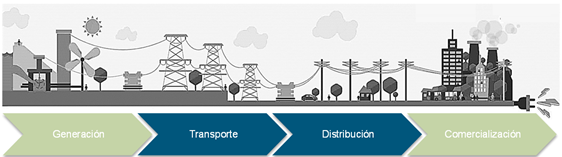
\includegraphics[width=1\textwidth]{Images/tfm-2.1.png}
    \caption{Actividades del sector eléctrico (\cite{yem-energy})}
    \label{fig:sec_elec}
\end{figure}

\subsection{Factores influyentes en la demanda eléctrica}

La predicción de la demanda eléctrica abarca un conjunto de variables, tanto conocidas como desconocidas, provenientes de una gran diversidad de orígenes. En el contexto de las series temporales, estas variables se definen como exógenas. Se refieren a un conjunto de factores que influyen en la magnitud de interés, pero que no son a su vez afectados por la misma. Estas variables provienen de fuentes externas, y su adecuada selección puede impulsar una mejora sustancial en los resultados. En el ámbito de la demanda eléctrica, existen numerosas variables exógenas, destacando los siguientes grupos:

\begin{itemize}
    \item \textbf{Variables temporales:} Elementos que abarcan diferentes intervalos de tiempo. Estas variables incluyen factores de estacionalidad y períodos vacacionales, así como días laborales y no laborales. Además, en intervalos de tiempo más pequeños, como por horas, se pueden analizar ciertos patrones de comportamiento de la demanda eléctrica:
    \begin{enumerate}
        \item Por estaciones (trimestrales).
        \item Por meses y semanas.
        \item Por días de la semana.
        \item Por días festivos.
    \end{enumerate}
    
\end{itemize}

\begin{itemize}
    \item \textbf{Variables climáticas:} conjunto de magnitudes directamente relacionadas con las condiciones atmosféricas.
    \begin{enumerate}
        \item Temperatura.
        \item Humedad.
        \item Otros factores: precipitaciones, velocidad del viento, entre otros.
        
    \end{enumerate}
    
\end{itemize}

\begin{itemize}
    \item \textbf{Factores económicos:} El precio de la electricidad influye directamente en la economía. Algunas variables económicas, por lo tanto, mantienen una relación significativa con la demanda eléctrica.
    \begin{enumerate}
        \item Producto interior bruto (PIB).
        \item Inflación.
        \item Mercado laboral.
        
    \end{enumerate}
    
\end{itemize}

No es posible abarcar la totalidad de las variables involucradas debido a la complejidad del problema. Solo se han presentado los grupos de variables más relevantes, junto con los ejemplos más utilizados en la bibliografía revisada. En este proyecto, no se consideran todos los ejemplos descritos, sino aquellos que tienen una mayor relación y, por ende, ofrecen mejores resultados.


\section{Fundamentos de las series temporales}

Una serie temporal ($Y_t$) es una sucesión de observaciones de variables registradas en diferentes instantes de tiempo. El análisis de series temporales es el proceso mediante el cual se busca descubrir el patrón o la tendencia de los datos, siguiendo tres fases: análisis exploratorio, elección de modelo y diagnóstico. En esta sección, únicamente se aborda la primera fase, ya que es fundamental para comprender el análisis que se desarrolla más adelante (\cite{rojasjimenez2022}).

Para iniciar con el análisis exploratorio, es fundamental comprender el concepto de descomposición de series temporales. Este término se refiere al conjunto de técnicas que permiten desglosar las diferentes componentes de las series, destacándose principalmente cuatro:

\begin{itemize}
    \item \textbf{Tendencia ($T_t$)}: patrón, no necesariamente lineal, de la dirección a largo plazo de la serie. Puede ser creciente, decreciente o estable.

    \item \textbf{Estacionalidad ($S_t$)}: fluctuaciones periódicas y regulares en intervalos de tiempo, causadas principalmente por factores estacionales como horas, días o meses.

    \item \textbf{Ciclicidad ($C_t$)}: similar a la estacionalidad, pero sin ocurrir en ciclos fijos o regulares. Comúnmente se combina con la tendencia.

    \item \textbf{Aleatoreidad o ruido ($R_t$)}: fluctuaciones irregulares que no siguen un patrón que se pueda identificar.
\end{itemize}

En la Figura \ref{fig:componentesST} se presenta la serie temporal completa (observada), junto con la tendencia y la ciclicidad (trend), la estacionalidad (seasonal) y la aleatoriedad (random). Esta figura es solo un ejemplo y no es necesario prestar atención a las magnitudes.

\begin{figure}[H]
    \centering
    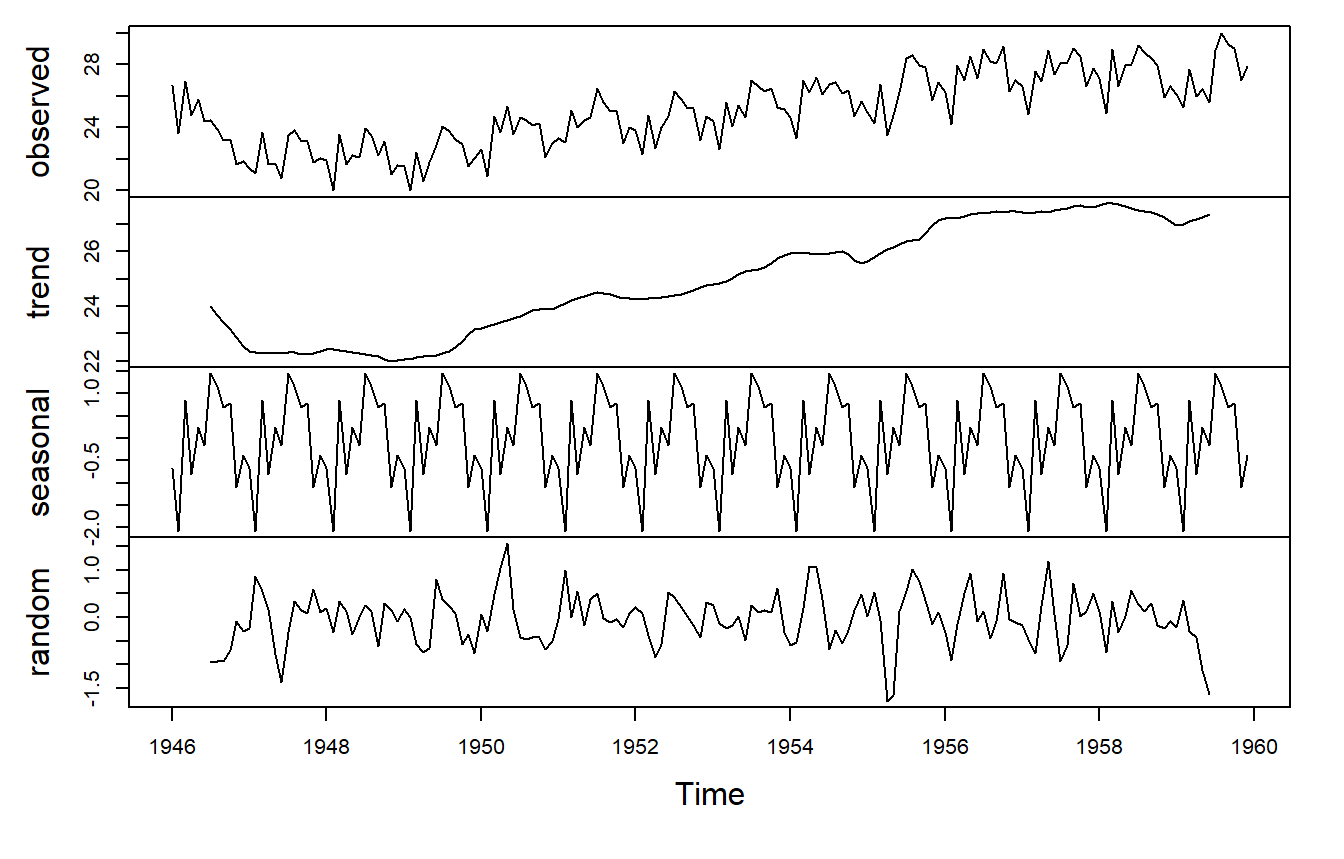
\includegraphics[width=1\textwidth]{Images/tfm-2.2.png}
    \caption{Componentes de una serie temporal de ejemplo \parencite[]{rojasjimenez2022}}
    \label{fig:componentesST}
\end{figure}

Para realizar la descomposición de series temporales se debe seguir un modelo o esquema de agregación. Los tres modelos más utilizados son:

\begin{itemize}
    \item \textbf{Modelo aditivo:} se basa en la suma de las tres componentes de la serie temporal.

    \begin{equation*}
        Y_t = T_t + S_t + R_t
    \end{equation*}

     \item \textbf{Modelo multiplicativo:} es el producto de las tres componentes.

     \begin{equation*}
        Y_t = T_t \times S_t \times R_t
    \end{equation*} 

    \item \textbf{Modelo mixto:} se trata de la combinación de los dos modelos previos.

     \begin{equation*}
        Y_t = T_t \times S_t + R_t
    \end{equation*}
\end{itemize}

\subsection{Estacionariedad de una serie temporal}

Uno de los conceptos más importantes en el análisis de series temporales es la estacionariedad. Una serie de tiempo se considera estacionaria si sus propiedades estadísticas no dependen del tiempo. Existen dos tipos de estacionariedad: la estacionariedad fuerte, que implica que la distribución de probabilidad se mantiene constante a lo largo del tiempo, y la estacionariedad débil, que se refiere a que el primer y el segundo momento de la distribución (es decir, la media y la varianza, respectivamente) no dependen del tiempo.

Las series temporales estacionarias son más fáciles de predecir, aunque es común que no se trabaje exclusivamente con este tipo. Además, es importante no confundir el término de estacionariedad con estacionalidad, ya que son conceptos complementarios pero distintos. 

El procedimiento más usado para determinar si una serie es estacionaria es la aplicación de la prueba Augmented Dickey-Fuller (ADF) (\cite{jacomeGarcia2024}). Esta técnica estadística tiene dos hipótesis:

\begin{itemize}
    \item \textbf{Hiótesis nula (H0)}: la serie temporal no es estacionaria.

    \item \textbf{Hiótesis nula (H1)}: la serie temporal es estacionaria.
\end{itemize}

Su metodología se basa en comparar la serie temporal con su versión diferenciada. Sí la serie no fuese estacionaria, la aplicación de una diferenciación exhibirá comportamientos estacionarios. Los valores usados en este tipo de análisis son:

\begin{itemize}
    \item \textbf{Estadística ADF}: medida que indica la lejanía de la serie temporal a ser no estacionaria. Conforme el valor es más negativo, mayor evidencia hay en contra de la hipótesis nula.

    \item \textbf{Valor \textit{p}}: probabilidad de observar los datos obtenidos (o más extremos) si la hipótesis nula de que la serie temporal es verdadera; un valor \textit{p} bajo sugiere que se puede rechazar la hipótesis nula.

    \item \textbf{Valores críticos}: umbrales que se utilizan para decidir si se debe rechazar la hipótesis nula, comparando con la estadística ADF.
\end{itemize}

Aunque el promedio y la varianza desempeñan un papel fundamental en el análisis exploratorio de series temporales, al representar la ubicación central y la dispersión de los datos, hay otra propiedad importante a considerar: la autocorrelación. Esta se define como la correlación de una variable consigo misma en diferentes momentos en el tiempo. En particular, se habla de autocorrelación de segundo orden, que se refiere a la correlación que únicamente depende del número de pasos que separan las observaciones, conocidos como lags (\cite{alvaroTruchado2024}). La elección adecuada del número de lags impacta significativamente en la calidad de los resultados predichos por los modelos.

Además, es esencial no olvidar un concepto complementario a la autocorrelación: la autocorrelación parcial. Esta mide la correlación entre la serie y un rezago específico, similar a la autocorrelación, pero controlando la influencia de los rezagos intermedios. Ambas herramientas son cruciales para analizar el comportamiento de la serie y realizar una elección adecuada de los lags a utilizar en los modelos.


\section{Modelos de series temporales}

\subsection{Modelos ARIMA y ARIMAX}

Los modelos Auto-Regressive Integrated Moving Average, o ARIMA, son uno de los conjuntos de modelos más utilizados para el pronóstico de series temporales estacionarias. Aunque estos modelos están diseñados para series estacionarias, también pueden aplicarse a series no estacionarias si se transforman adecuadamente. Esto se puede lograr mediante técnicas como la diferenciación o a través de transformaciones no lineales. Los modelos ARIMA combinan tres componentes:

\begin{itemize}
    \item \textbf{AR (autoregresivo)}: utiliza valores rezagados de la variable dependiente u objetivo.

    \item \textbf{I (integrado)}: diferencias aplicadas para hacer la serie estacionaria.

    \item \textbf{AR (media móvil)}: utiliza valores retrasados de los errores.
\end{itemize}

En resumen, un modelo ARIMA(\textit{p},\textit{d},\textit{q}) es un algoritmo de predicción de series temporales que usa la combinación de valores pasados y errores pasados. Las variables de la función son:

\begin{itemize}
    \item \textbf{\textit{p}}: número de términos autoregresivos.

    \item \textbf{\textit{d}}: cantidad de diferencias necesarias para la estacionariedad.

    \item \textbf{\textit{q}}: número de errores rezagados.
\end{itemize}

Para comprender de manera adecuada el modelo, es necesario mostrar la ecuación general:

\begin{equation*}
    Y_t = \mu + \sum_{i=1}^{p} \phi_i Y_{t-i} - \sum_{j=1}^{q} \theta_j e_{t-j} + e_t
\end{equation*}

\

Donde:

\begin{itemize}
    \item $Y_t$ es el valor predicho en el tiempo $t$.

    \item $\mu$ es la media de la serie.

    \item $\phi_1$, ..., $\phi_p$ son los parámetros autoregresivos.

    \item $\theta_1$, ..., $\theta_p$ son los parámetros de media móvil.

    \item $e_{t-1}$, ..., $e_{t-q}$ son los errores rezagados de predicciones pasadas.
\end{itemize}

Por lo que se puede confirmar que la parte más importante al aplicar un modelo ARIMA(\textit{p},\textit{d},\textit{q}) es la determinación de las constantes \textit{p}, \textit{d} y \textit{q} (\cite{nau2024}).

Hasta ahora no se han tenido en cuenta las variables exógenas ya que el modelo ARIMA(\textit{p},\textit{d},\textit{q}) únicamente funciona con la variable independiente del tiempo. Para poder incorporar nuevas variables independientes se crea la variación ARIMAX(\textit{p},\textit{d},\textit{q}). Debido a la posibilidad de implementar variables exógenas, esta extensión mejora los resultados del algoritmo original capturando nuevos comportamientos y patrones complejos relacionados con las nuevas variables. Esto es útil cuando las dependencias no pueden ser explicadas totalmente mediante relaciones internas de la serie. Aunque esto puede ser un arma de doble filo, ya que incorporar variables exógenas con relaciones bajas con la variable objetivo puede perjudicar de manera sustancial los resultados. Es importante la elección previa de variables a tratar para garantizar unos mejores resultados. La ecuación general de este modelo es:

\begin{equation*}
    Y_t = \mu + \sum_{i=1}^{p} \phi_i Y_{t-i} - \sum_{j=1}^{q} \theta_j e_{t-j} + \sum_{k=1}^{r} \beta_k X_{t-k} + e_t
\end{equation*}

Donde, considerando únicamente las nuevas variables:

\begin{itemize}
    \item $X_{t-k}$ son las variables exógenas con $k = 1$, ..., $r$. $r$ es el número total.

    \item $\beta_k$ son los coeficientes de las variables exógenas.
\end{itemize}

En resumen, este modelo es similar a su antecesor solo que añade una componente que incorpora el efecto de variables exógenas (\cite{jacomeGarcia2024}).

\subsection{Forecaster autoregresivo}

Los modelos autoregresivos (AR) conforman una parte del modelo ARIMA, destinada a la predicción de valores futuros mediante la combinación lineal de varios valores pasados. Es decir, la fórmula descriptiva corresponde a los términos asociados a los parámetros autoregresivos y el error rezagado:

\begin{equation*}
    Y_t = \sum_{i=1}^{p} \phi_i Y_{t-i} + e_t
\end{equation*}


A pesar de que en primera instancia estos modelos trabajan con algoritmos lineales, se pueden implementar otro tipo de algoritmos más sofisticados que tengan en cuenta relaciones más complejas. Para ello, se puede generalizar la función de la expresión anterior:

\begin{equation*}
    Y_t = f(Y_{t-1}, Y_{t-2}, \dots, Y_{t-p}) + \varepsilon_t
\end{equation*}

Donde:

\begin{itemize}
    \item $Y_t = f(Y_{t-1}, Y_{t-2}, \dots, Y_{t-p}) + \varepsilon_t$ es el regresor o algoritmo generalizado.
    \item $e_{t-}$ es el error en el instante $t$.
\end{itemize}

De esta manera, se pueden utilizar una gran variedad de técnicas de predicción más avanzadas, incluyendo algoritmos de Machine Learning.

\subsection{Backesting}

En el contexto de los sistemas de predicción, el overfitting es un fenómeno que ocurre cuando el modelo se ajusta demasiado a los datos de entrenamiento, captando ruido y volviéndose excesivamente complejo. Este ajuste excesivo resulta en una pérdida de generalización del modelo, lo que conduce a predicciones engañosas y poco precisas.


Para combatir el overfitting, se emplean diversas técnicas de validación, entre ellas la validación cruzada o cross-validation (Figura \ref{fig:cross_val}). Esta técnica implica dividir el conjunto de entrenamiento en \textit{K} subconjuntos de tamaños similares, conocidos como pliegues (folds). El modelo se entrena utilizando \textit{K} - 1 subconjuntos y valida su rendimiento con el restante. Este proceso se repite un número \textit{K} de veces (\cite{gonzalezdorado2024ML}). Sin embargo, este enfoque tradicional no se puede aplicar directamente a las series temporales debido a la naturaleza secuencial de los datos. Existen otras metodologías que ayudan a controlar el overfitting: selección adecuada de las características (en este caso variables exógenas), controlar el entrenamiento de los modelos para evitar que sean demasiado complejos y uso de una mayor cantidad de datos.

\begin{figure}[H]
    \centering
    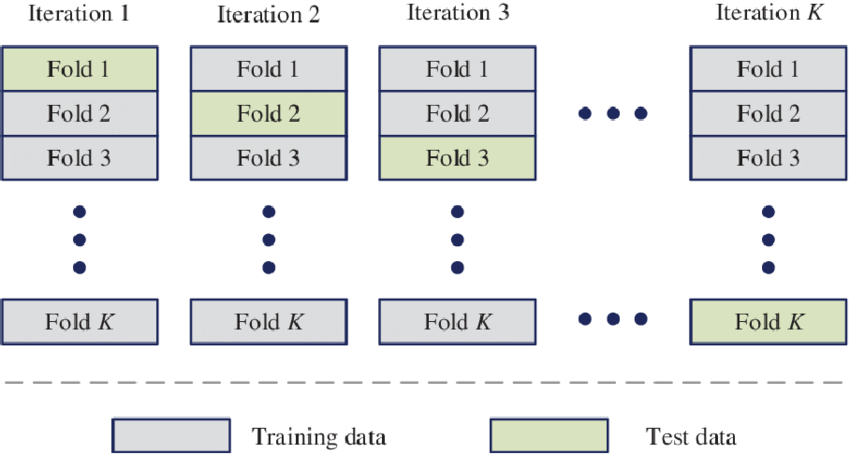
\includegraphics[width=0.75\textwidth]{Images/tfm-2.4.png}
    \caption{Validación cruzada (\cite{researchgate_figura3-4})}
    \label{fig:cross_val}
\end{figure}

De la necesidad de adaptar la validación cruzada a los problemas de series temporales, surge el backesting, un tipo especial de validación cruzada que se aplica a periodos previos (\cite{skforecast}). El backesting consiste en evaluar las predicciones del modelo a través de una visión retrospectiva de los datos históricos. Se pueden utilizar diversas técnicas de backesting, cuya elección dependerá de las necesidades específicas del problema de series temporales que se esté abordando. Las principales técnicas de backesting son:

\begin{itemize}
    \item \textbf{Backesting sin reajuste}: el modelo se entrena una sola vez y se actualiza de forma secuencial sin actualizarlo, siguiendo el orden natural de los datos (Figura \ref{fig:bck1}). Es la técnica más rápida, pero puede perder precisión en los resultados al no utilizar los últimos valores predichos.

    \begin{figure}[H]
    \centering
    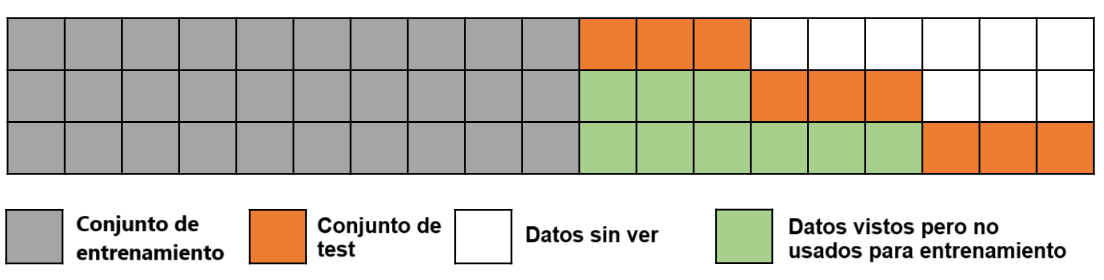
\includegraphics[width=0.75\textwidth]{Images/tfm-2.11.png}
    \caption{Diagrama-esquema de backesting sin reajuste (\cite{skforecast})}
    \label{fig:bck1}
    \end{figure}

    \item \textbf{Backesting con reajuste y aumento del tamaño de entrenamiento}: el modelo se entrena reincorporando los últimos valores predichos y aumenta el tamaño del conjunto de entrenamiento (Figura \ref{fig:bck2}). Es decir, la cantidad de datos históricos va aumentando de forma secuencial, mejorando la capacidad predictiva del modelo. Esta técnica tiene altos costes computacionales.

    \begin{figure}[H]
    \centering
    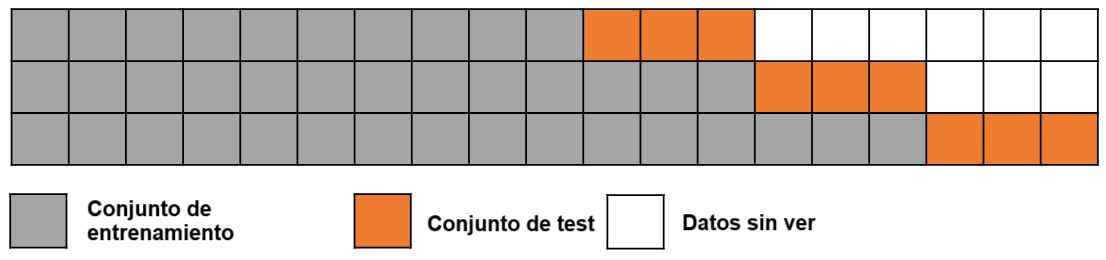
\includegraphics[width=0.75\textwidth]{Images/tfm-2.12.png}
    \caption{Diagrama-esquema de backesting con reajuste y aumento del tamaño de entrenamiento (\cite{skforecast})}
    \label{fig:bck2}
    \end{figure}
    
    \item \textbf{Backesting con reajuste y tamaño de entrenamiento fijo}: utiliza el concepto de ventana fija, donde el tamaño del conjunto de entrenamiento se mantiene constante y avanza en el tiempo (Figura \ref{fig:bck3}). Esta técnica es útil cuando el rendimiento del modelo puede variar según el tiempo, normalmente cuando hay una cantidad de datos limitada o la serie no es estacionaria. Es la técnica que más se asemeja a la validación cruzada tradicional, solo que en series temporales. 

    \begin{figure}[H]
    \centering
    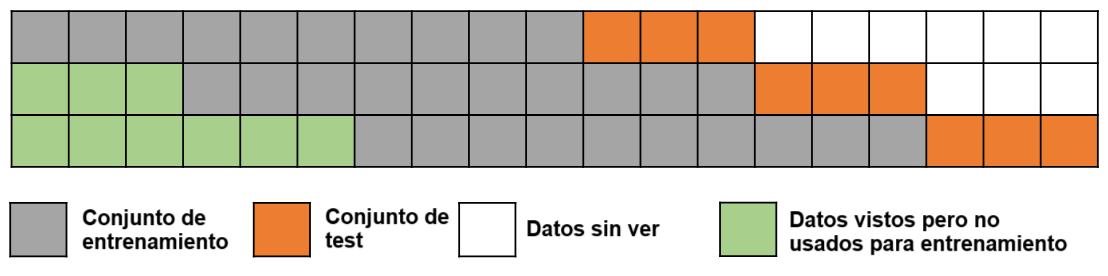
\includegraphics[width=0.75\textwidth]{Images/tfm-2.13.png}
    \caption{Diagrama-esquema de backesting con reajuste y tamaño de entrenamiento fijo (\cite{skforecast})}
    \label{fig:bck3}
    \end{figure}
    
\end{itemize}


\section{Machine Learning}

El Machine Learning o aprendizaje automático, es una rama de la inteligencia artificial que se basa en la capacidad de los sistemas informáticos para aprender de los datos sin seguir instrucciones programadas de forma explícita. Destacan dos grupos de técnicas:

\begin{itemize}
    \item \textbf{Aprendizaje no supervisado}: técnicas con la que se busca explorar la estructura de un conjunto de datos para encontrar patrones de comportamiento. Las variables no tienen por qué estar etiquetadas para extraer el conocimiento. Donde una variable etiquetada es un tipo de dato que incluye una un valor de referencia asociado, que indica su categoría o resultado.

    \item \textbf{Aprendizaje supervisado}: conjunto de técnicas que tienen como fin la predicción de una variable objetivo mediante un conjunto de datos previamente etiquetados. Dependiendo de las características de la variable objetivo se subdividen en modelos de clasificación (variable discreta) o predicción (variable continua).
\end{itemize}

Debido a las características del proyecto, las técnicas a usar se basan en aprendizaje supervisado de tipo predictivo. Este conjunto de algoritmos sigue una lógica de aprendizaje inherente. La Figura \ref{fig:MLSup} muestra esquemáticamente y de manera resumida el funcionamiento de las técnicas de aprendizaje supervisado. Las diferentes variables etiquetadas y la variable etiqueta (objetivo) son preprocesadas y adaptadas para poder inferir sobre el modelo de predicción. Se debe realizar una división previa del conjunto de datos en dos: un conjunto de entrenamiento, con el cual se entrena el modelo, y un conjunto de prueba, que, sin variable objetivo, sirve para evaluar el rendimiento del modelo una vez entrenado.

\begin{figure}[H]
    \centering
    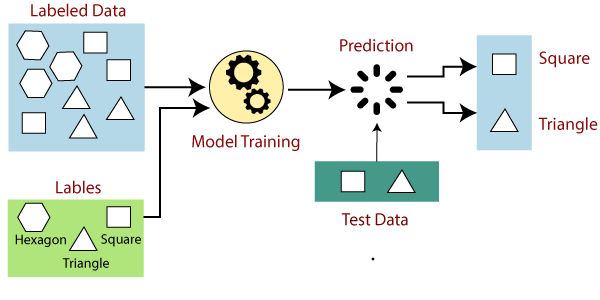
\includegraphics[width=1\textwidth]{Images/tfm-2.3.png}
    \caption{Esquema de técnica de aprendizaje supervisado (\cite{javatpoint_supervised_ml})}
    \label{fig:MLSup}
\end{figure}

Cada modelo depende de una serie de características denominadas hiperparámetros: parámetros inherentes al modelo cuyo valor influye en el rendimiento y la capacidad de generalización de los resultados, es decir, en la calidad de las predicciones. Además, cuando se evalúa la calidad de un modelo o un ajuste, es importante medir el error en función de diversas métricas, como el Mean Squared Error (MSE), el Root Mean Squared Error (RMSE) y el Mean Absolute Error (MAE). En la Tabla \ref{tbl:metrics} se muestra cada métrica con una breve descripción y su fórmula (\cite{arrioja2021}). En cada expresión matemática:

\begin{itemize}
    \item $n$ es el número total de datos.
    \item $y_i$ valor real de la variable objetivo en la iteración $i$.
    \item $\hat{y_i}$ valor predicho de la variable objetivo en la iteración $i$.
    \item $y_i - \hat{y_i}$ diferencia del valor real y el predicho (error).
\end{itemize}


\begin{table}[H]
\centering
\caption{\\ Métricas de evaluación de modelos}
\renewcommand{\arraystretch}{1.5} % Incrementa el espacio entre filas dentro de la tabla
\begin{tabular}{>{\raggedright\arraybackslash}p{2.5cm} >{\raggedright\arraybackslash}p{9cm} >{\raggedright\arraybackslash}p{3.5cm}}
\toprule
\textbf{Métrica} & \textbf{Descripción} & \textbf{Fórmula} \\ 
\midrule
\textbf{MSE}   & Media de los errores al cuadrado. Penaliza los errores más grandes (outliers). & \( \frac{1}{n} \sum_{i=1}^{n} ( y_i - \hat{y}_i )^2 \) \\ \hline
\textbf{RMSE}  & Raíz cuadrada del MSE. Es más interpretable ya que sus unidades corresponden con las de la variable objetivo. & \( \sqrt{ \frac{1}{n} \sum_{i=1}^{n} ( y_i - \hat{y}_i )^2 } \) \\ \hline
\textbf{MAE}   & Media de los errores absolutos. Es más robusta frente a valores atípicos y es la más sencilla de comprender. & \( \frac{1}{n} \sum_{i=1}^{n} \left| y_i - \hat{y}_i \right| \) \\
\bottomrule
\end{tabular}
\renewcommand{\arraystretch}{1} % Restablece el espaciado predeterminado después de la tabla
\label{tbl:metrics}
\caption*{\textit{Nota}: (Elaboración propia)}
\end{table}



\subsection{Árboles de decisión}

Los árboles de decisión (Decision Tree) son una técnica de aprendizaje automático que permite identificar conceptos a partir de las características de un conjunto de datos de entrenamiento. Su nombre se debe al sistema jerárquico de los resultados, basado en un grafo dirigido con nodos y arcos, cuya figura puede recordar a un árbol. Los nodos son las conexiones entre las ramificaciones y pueden concebirse como preguntas que se basan en una variable del conjunto de entrenamiento, cuya respuesta clasifica los resultados. Tanto las preguntas formuladas como el orden en que se ejecutan son importantes. La Figura \ref{fig:DT} ejemplifica de manera visual los conceptos mencionados.

\begin{figure}[H]
    \centering
    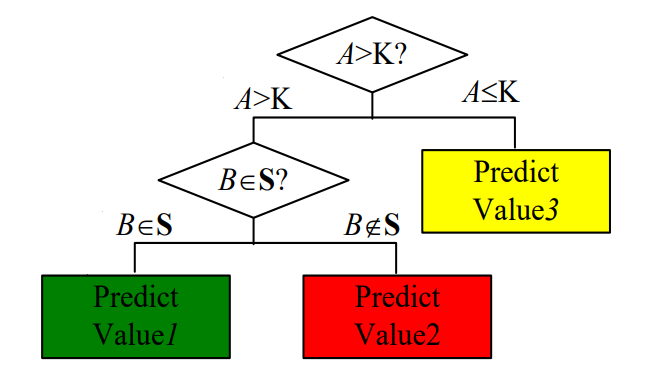
\includegraphics[width=0.6\textwidth]{Images/tfm-2.5.png}
    \caption{Esquema de árbol de decisión (\cite{liu2013overview})}
    \caption*{\textit{Nota}: Donde $A$ y $B$ son variables del conjunto de entrenamiento y $K$ y $S$ constantes cualquiera}
    \label{fig:DT}
\end{figure}

En el caso de los árboles de decisión, los hiperparámetros principales son:

\begin{itemize}
    \item \textbf{Maximum depht}: máxima profundidad del árbol.

    \item \textbf{Maximum branch}: número de ramas máximo en las que se puede dividir un nodo.

    \item \textbf{Leaf size}: número mínimo de observaciones por nodo final para que se construya la regla.

    \item \textbf{Split size}: número mínimo de observaciones para dividir un nodo.

    \item \textbf{Discriminant variables}: proceso de parada por no encontrar una variable lo suficientemente discriminante.
\end{itemize}

Este conjunto de algoritmos sigue un método específico. Primero, se calcula la calidad (información) del nodo; si este no cumple con los estándares, se determina el mejor atributo separador. De esta manera, se añade a la base de reglas y se divide el conjunto inicial en al menos otros dos, pero con mayor calidad. Se realizan iteraciones hasta que se alcance un criterio de parada: profundidad máxima, número mínimo de observaciones por nodo, entre otros.

En conclusión, los árboles de decisión son uno de los conjuntos de algoritmos más utilizados en Machine Learning. Su concepto sencillo y el rendimiento comparable al de otros modelos más complejos respaldan su uso en numerosos estudios basados en la predicción de una variable objetivo. No obstante, la mayor desventaja se manifiesta en conjuntos de datos más complejos, donde los árboles generados son tan grandes y profundos que resultan casi imposibles de entender y son propensos a un sobreaprendizaje severo. Puede ser un buen punto de partida su aplicación en el caso de la predicción de series temporales, ya que es adecuada para identificar patrones complejos en los datos de manera intuitiva y adaptable.


\subsection{Conjuntos de modelos}

Para abordar la problemática del sobreajuste en los árboles de decisión, han surgido diversas técnicas denominadas métodos de ensamblado (ensemble methods). En general, estas técnicas se basan en la combinación de múltiples modelos de árboles de decisión para mejorar el rendimiento de cada modelo individual. De esta manera, se puede reducir el error asociado con la aproximación de una función compleja a un modelo excesivamente simple, así como la varianza (es decir, la capacidad de adaptación en distintos conjuntos de entrenamiento). Este tipo de técnicas son ideales para la predicción de series temporales, ya que la combinación de múltiples modelos mejora la precisión y captura de manera más efectiva las fluctuaciones y patrones complejos en los datos.

En cuanto a las ventajas, el promedio de los errores de cada modelo mejora los resultados en comparación con si actuara de manera individual; hay menor sobreajuste, ya que son menos sensibles a los datos de entrenamiento (como los valores atípicos) y pueden aumentar significativamente el rendimiento. Dentro de este tipo de técnicas, destacan dos grupos: Bagging y Boosting, como se muestra en la Figura \ref{fig:BB}.


\begin{figure}[H]
    \centering
    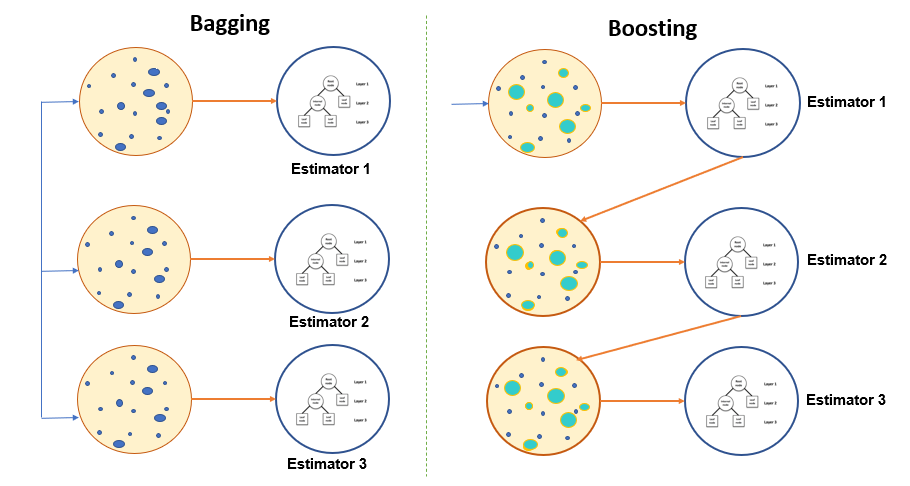
\includegraphics[width=1\textwidth]{Images/tfm-2.6.png}
    \caption{Esquema de los modelos de Bagging y Boosting (\cite{liu2013overview})}
    \label{fig:BB}
\end{figure}

\subsubsection{Bagging}

La técnica Bagging, o también conocido como Bootstrap Aggregation, crea cada árbol individual a partir de una muestra aleatoria de los datos de entrenamiento, manteniéndose el tamaño por defecto. Básicamente se mantiene la cantidad de datos pero no la composición. Los modelos son entrenados de forma paralela y los resultados de la predicción son en el promedio de las predicciones individuales.

Una extensión del Bagging muy utilizada es el Random Forest. Este algoritmo sigue una estrategia similar a su predecesor, pero añade un elemento más de aleatoriedad. En el proceso de composición de los datos de entrenamiento, se realiza una selección aleatoria de los atributos a estudiar. Estos nuevos subconjuntos se conocen como random subspaces. En el caso del Random Forest, se añaden a los hiperparámetros del árbol de decisión (\cite{sklearn_random_forest_regressor}) los siguientes:

\begin{itemize}
    \item \textbf{Number of estimators}: cantidad de árboles.

    \item \textbf{Maximum features}: máximo número de atributos considerados para crear los random subspaces.

    \item \textbf{Maximum samples}:  máximo número de muestras del conjunto de entrenamiento que se usan para entrenar cada árbol.
\end{itemize}

\subsubsection{Boosting}

Este algoritmo sigue un enfoque alternativo a los antes mencionados, ya que está formado por una estructura secuencial basada en weak learners. En este contexto, los weak learners son árboles de decisión muy simples y con poca profundidad. Estos en un contexto individual pueden generar predicciones erráticas e incluso aleatorios ya que están concebidos para trabajar de manera secuencial. Cada modelo individual intenta corregir los errores cometidos en la iteración previa mediante la optimización de una función de pérdida (diferencia de las predicciones con los valores reales).

Uno de los algoritmos más utilizados en este contexto es el XGBoost (Extreme Gradient Boosting). Se basa en la técnica de boosting por gradiente, donde en cada iteración se calcula el gradiente de la función de pérdida (diferencia entre las predicciones y los valores reales) de la iteración anterior. Conforme avanza la secuencia, se minimiza dicha función, lo que hace que las siguientes iteraciones sean más precisas y el modelo mejore progresivamente. Además, incorpora técnicas de regularización que ayudan a evitar el sobreajuste. XGBoost es un modelo altamente escalable, diseñado para trabajar en sistemas distribuidos, lo que lo hace especialmente atractivo para manejar grandes volúmenes de datos. Sus hiperparámtros más importantes, sin mencionar los explicados en los árboles de decisión (\cite{sklearn_random_forest_regressor}):

\begin{itemize}
    \item \textbf{Number of estimators}: cantidad de árboles.

    \item \textbf{Learning rate}: tasa de aprendizaje (cuanto se ajusta el modelo en cada iteración).

    \item \textbf{Objective}: función de pérdida.

    \item \textbf{Gamma}: reducción mínima en la función de pérdida que se necesita para realizar una partición adicional en un nodo.

    \item \textbf{Alpha}: término de regularización para prevenir el sobreajuste.

    \item \textbf{Lambda}: otro término de regularización para prevenir el sobreajuste.
    
    \item \textbf{Subsample ratio of the training instances}: proporción de datos para entrenar cada árbol.

    \item \textbf{Subsample ratio of columns when constructing each tree}: fracción de características que se utilizarán para construir cada árbol. 
\end{itemize}

\section{Introducción al Deep Learning}

El Deep Learning (aprendizaje profundo) es una rama del Machine Learning que busca replicar el funcionamiento del cerebro humano para procesar, razonar y aprender. Esta tecnología se fundamenta en el uso de redes neuronales artificiales profundas, lo que da origen al término deep (profundo).

Una red neuronal artifical está conformada por dos elementos principales y complementarios (\cite{gonzalezdorado2024DP}):

\begin{itemize}
    \item \textbf{Neurona}: unidad fundamental de la red neuronal, representada en forma de nodo. Procesa una serie de entradas para dar una salida.

    \item \textbf{Capa}: conjunto de neuronas en paralelo. Una red neuronal está conformada por varias capas de neuronas. Existen tres tipos fundamentales:

        \begin{enumerate}
            \item \textbf{Capa de entrada}: neuronas que reciben los datos (input).

            \item \textbf{Capa oculta}: neuronas intermedias que acarrean la mayor parte del procesamiento. Estas capas son las responsables de aprender y capturar patrones, es decir, son la parte central del algoritmo.

            \item \textbf{Capa de entrada}: neuronas que proporcionan la respuesta (output).
        \end{enumerate}
\end{itemize}

\begin{figure}[H]
    \centering
    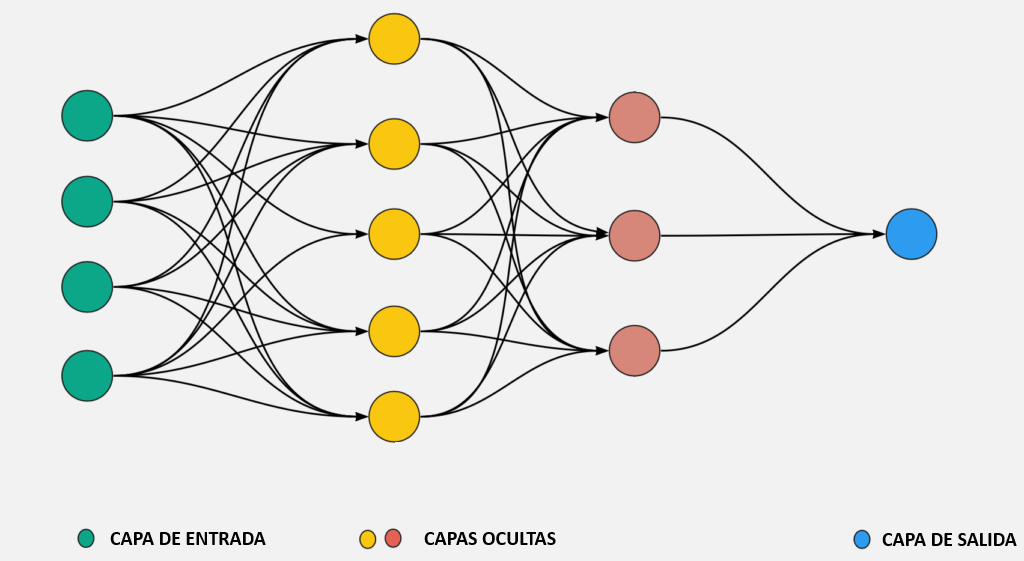
\includegraphics[width=0.9\textwidth]{Images/tfm-2.9.png}
    \caption{Esquema de las capas de una red neuronal (\cite{fouzan2023understanding})}
    \label{fig:ANN}
\end{figure}

La Figura \ref{fig:ANN} esquematiza los conceptos mencionados. Aunque se ha explicado la estructura básica de una red neuronal, es necesario introducir el concepto de peso: un valor numérico que representa la importancia de la conexión entre dos neuronas. Si la diferencia entre la salida proporcionada por la neurona y la salida esperada no es lo suficientemente pequeña, se ajustan los pesos para mejorar los resultados del modelo. Este proceso es iterativo hasta que se alcanza la salida con la precisión deseada. La diferencia entre ambas salidas se calcula mediante la función de pérdida.

Las funciones que capturan los patrones en los datos y determinan si una neurona debe activarse se denominan funciones de activación. Existen dos tipos principales: lineales y no lineales. Las funciones lineales generan una salida directamente proporcional a la entrada, pero no pueden aprender patrones complejos. En cambio, las funciones no lineales permiten a la red neuronal captar relaciones más complejas, lo que las hace esenciales para resolver problemas más avanzados. Algunos ejemplos de funciones no lineales son la tangente hiperbólica y la sigmoide. Las funciones de activación suelen ir acompañadas de otro concepto: el sesgo, que es un valor adicional que se suma a las entradas de las neuronas con el fin de ajustar la salida, incluso cuando la entrada es nula (\cite{jacomeGarcia2024}).


\subsection{Redes neuronales recurrentes. RNN y LSTM}

Las redes neuronales recurrentes (RNN) son un tipo de red neuronal diseñada para procesar datos con un orden secuencial, lo que las hace muy útiles para la predicción de series temporales. Las redes neuronales tradicionales siguen un único sentido en la transmisión de la información, mientras que las RNN mantienen estados de memoria internos que permiten recordar y tener en cuenta información pasada. La unidad fundamental es la célula recurrente, la cual toma dos entradas: la actual y la del estado oculto previo. La Figura \ref{fig:RNN} representa esquemáticamente este tipo de redes neuronales.

\begin{figure}[H]
    \centering
    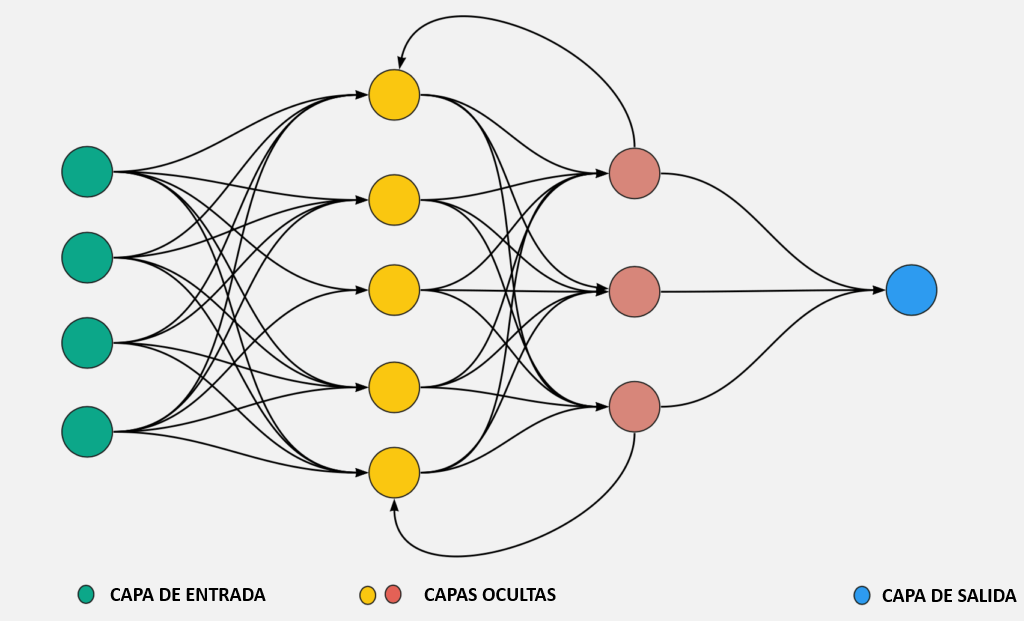
\includegraphics[width=0.9\textwidth]{Images/tfm-2.10.png}
    \caption{Esquema de las capas de una red neuronal recurrente (\cite{fouzan2023understanding})}
    \label{fig:RNN}
\end{figure}

A pesar del gran potencial de las RNN, se observan ciertas limitaciones al capturar patrones a largo plazo. Para ello surgen una serie de variantes que mejoran sustancialmente estas problemáticas, destacando las redes neuronales Long Short-Term Memory (LSTM) (\cite{skforecast}). Incorporan una arquitectura más compleja conformada por una estructura modular de tres puertas (gates):

\begin{itemize}
    \item \textbf{Puerta de olvido (Forget gate)}: regula la cantidad de información a olvidar, combinando la entrada actual con la salida anterior.

    \item \textbf{Puerta de entrada (Input gate)}: regula la información a añadir en la memoria a largo plazo.

    \item \textbf{Puerta de salida (Output gate)}: regula que cantidad de información de la memoria actual se utilizará para el output final. Combina la entrada actual con la información de la memoria.
\end{itemize}

Al igual que cualquier algoritmo de Machine Learning, los modelos LSTM tienen una serie de hiperparámetros propios. A pesar de que su número es elevado, se resumen los más importantes:

\begin{itemize}
    \item \textbf{Number of layers}: número de capas que se apilan una encima de otras.

    \item \textbf{Number of units per Layer}: cantidad de neuronas por capa.

    \item \textbf{Learning rate}: tasa de rapidez en la actualización de pesos.

    \item \textbf{Activation function}: función de activación.

    \item \textbf{Batch size}: número de muestras que se utilizan en cada iteración de actualización de pesos.

    \item \textbf{Number of epochs}: número total de veces que el modelo pasa por el conjunto de entrenamiento.

    \item \textbf{Regularization}: métodos para evitar el sobreajuste de la red neuronal.

    \item \textbf{Optimization algorithm}: algoritmo de optimización. Se usa principalmente la función Adam.

    \item \textbf{Weight Initialization configuration}: configuración inicial de los pesos.
\end{itemize}







\section{Optimización de hiperparámetros}

A la hora de entrenar los modelos y obtener predicciones, es muy importante la elección adecuada de los valores de los hiperparámetros según el algoritmo usado. Esto se debe a que todos los modelos necesitan una parametrización específica para que su comportamiento se ajuste de manera adecuada al contexto del problema en concreto. Existen numerosas técnicas que permiten optimizar los hiperparámetros para mejorar los resultados.


\subsection{Random Search}

La técnica Random Search se basa en la exploración del espacio de hiperparámetros mediante la selección de puntos aleatorios dentro de pequeños rangos. Sirve para explorar los datos y encontrar la zona aproximada donde se puede encontrar la mejor combinación de hiperparámetros (Figura \ref{fig:RSearch}). Los principales argumentos son el número de iteraciones y el número de combinaciones o cruces para la validación cruzada. Debido a su naturaleza, no funciona de manera adecuada con un número alto de iteraciones, lo que acarrea problemas de procesamiento.

\begin{figure}[H]
    \centering
    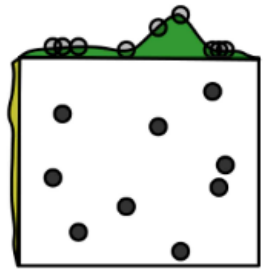
\includegraphics[width=0.3\textwidth]{Images/tfm-2.7.png}
    \caption{Espacio de hiperparámetros en Random Search (\cite{gonzalezdorado2024ML})}
    \label{fig:RSearch}
\end{figure}

\subsection{Grid Search}

La técnica Grid Search es un proceso de optimización de hiperparámetros basado en la segmentación y búsqueda metódica de combinaciones. Para ello, se divide el espacio en una cuadrícula de valores posibles y se evalúan todas las combinaciones de estos valores (Figura \ref{fig:GSearch}). Tiene el mismo problema que la técnica anterior, conforme el espacio o el número de segmentaciones aumenta, el rendimiento baja, provocando altos costes computacionales. 

\begin{figure}[H]
    \centering
    
\includegraphics[width=0.3\textwidth]{Images/tfm-2.8.png}
    \caption{Espacio de hiperparámetros en Grid Search (\cite{gonzalezdorado2024ML})}
    \label{fig:GSearch}
\end{figure}

\subsection{Optimización bayesiana}

Aunque las estrategias anteriores funcionan de manera satisfactoria en muchos casos, sobre todo cuando no hay una gran cantidad de hiperparámetros, presentan un inconveniente: no tienen en cuenta los resultados obtenidos hasta el momento. La optimización bayesiana corrige esta problemática, dirigiendo la optimización hacia las regiones del espacio de hiperparámetros donde se obtienen los mejores resultados. Es decir, se basa en crear un modelo probabilístico en el que el valor de la función objetivo se fundamenta en la métrica de validación del modelo. Esta estrategia permite que la búsqueda se dirija en cada iteración hacia las áreas más prometedoras. El objetivo final es reducir el número de combinaciones de hiperparámetros que se evalúan, seleccionando solo los mejores candidatos. Esto mejora el rendimiento, permitiendo explorar espacios con un elevado número de hiperparámetros (\cite{amat2020optimizacion}).



\chapter{Desarrollo}\label{cap:cap4}

El desarrollo del proyecto se ha llevado a cabo utilizando una metodología estructurada y previamente definida. Para una mejor comprensión y documentación de las ideas, se ha elegido el entorno de desarrollo \textit{Jupyter}, basado en notebooks de \textit{Python}. La metodología seguida contiene los siguientes puntos:

\begin{enumerate}
    \item \textbf{Extracción y preprocesamiento de datos}: proceso de elección de variables exógenas, extracción de datos de diferentes fuentes, unificación y preprocesamiento de datos.

    \item \textbf{Análisis exploratorio de datos (EDA)}: análisis de tipo de datos, estadística descriptiva básica, correlación de variables y análisis de series temporales.

    \item \textbf{Entrenamiento de modelos}: elección de los modelos, entrenamiento y optimización de hiperparámetros.
\end{enumerate}

Esta sección se centra en la explicación de la metodología seguida a lo largo del proyecto. El repositorio del código se encuentra en GitHub (\cite{gregorio}), adecuadamente ordenado y explicado. El proceso de visualización y análisis de resultados se desarrolla en la siguiente sección, que dará paso a la extracción de conclusiones en base a los objetivos propuestos con anterioridad.

\section{Extracción y preprocesamiento de los datos}

Uno de los aspectos importantes al estudiar y modelizar la demanda eléctrica es la elección adecuada de las variables exógenas que se integrarán con la variable objetivo. Dado que los objetivos del proyecto se centran menos en obtener resultados excepcionales y más en analizar el rendimiento de los algoritmos de predicción en diferentes escenarios, se ha optado por seleccionar las variables exógenas más influyentes en este contexto: variables temporales y climáticas, excluyendo las económicas. Las variables económicas tienen una influencia menor, ya que, en general, sus variaciones se observan en periodos de tiempo más largos. Las variables exógenas seleccionadas son:

\begin{itemize}
    \item \textbf{Día de la semana}.

    \item \textbf{Trimestre}.

    \item \textbf{Festivos}.

    \item \textbf{Temperatura}.

    \item \textbf{Humedad}.
\end{itemize}

Se anticipa que la variable humedad, debido a su baja relación directa con la demanda eléctrica, podría afectar negativamente los resultados de los modelos. Esto es una buena oportunidad para estudiar la influencia de variables exógenas que tienen relaciones débiles con la variable objetivo.

\subsection{Fuentes de datos. Extracción}

Una vez seleccionadas las variables necesarias, se lleva a cabo un estudio exhaustivo de las fuentes de datos disponibles y de su nivel de fiabilidad. En este caso, se han utilizado las APIs de dos entidades públicas: la Red Eléctrica Española (REE) (\cite{reeAPI}) y la Agencia Estatal de Meteorología (AEMET) (\cite{aemetAPI}). En ambos casos, fue necesario solicitar un API token personalizado, recibido vía correo electrónico.

De la API de la Red Eléctrica Española se han obtenido los datos principales de demanda eléctrica. Debido a la complejidad de los archivos \textit{JSON} de respuesta de esta API, se ha empleado una biblioteca no oficial de \textit{Python}, \textit{Pyesios} (\cite{pyesios}), compuesta por una serie de clases que permiten realizar consultas a la API de forma sencilla, mediante parámetros como la localización espacial, la frecuencia y el rango temporal.

La Tabla \ref{tbl:datos_demanda} muestra un ejemplo de los datos resultantes sin ser procesados, cuyas columnas son:

\begin{itemize}
    \item \textbf{datetime\_utc}: fecha en formato "YYYY-MM-DD HH:MM:SS$\pm$HH:MM".

    \item \textbf{Demanda real}: demanda eléctrica diaria a nivel peninsular ($MW$).

    \item \textbf{geo\_id}: localización geográfica, en este caso peninsular (\textit{geo\_id} = 8741).

    \item \textbf{año}: año en el que se hizo la medida.
\end{itemize}

\begin{table}[H]
\centering
\caption{\\ Datos del API de la REE extraídos y preprocesados} 
\renewcommand{\arraystretch}{1.3} % Incrementa el espacio entre filas dentro de la tabla
\begin{tabular}{llll}
\toprule
\textbf{datetime\_utc}       & \textbf{Demanda real} & \textbf{geo\_id} & \textbf{año} \\ \midrule
2018-12-31 00:00:00+00:00    & 23459,0               & 8741             & 2019         \\ \hline
2019-01-01 00:00:00+00:00    & 23083,58              & 8741             & 2019         \\ \hline
2019-01-02 00:00:00+00:00    & 29587,33              & 8741             & 2019         \\ \hline
2019-01-03 00:00:00+00:00    & 31287,31              & 8741             & 2019         \\ \hline
2019-01-04 00:00:00+00:00    & 31500,99              & 8741             & 2019         \\ \bottomrule
\end{tabular}
\renewcommand{\arraystretch}{1} % Restablece el espaciado predeterminado después de la tabla

\label{tbl:datos_demanda}
\caption*{\textit{Nota}: (Elaboración propia)}
\end{table}


Para extraer el resto de variables exógenas se ha usado la API pública del AEMET con la librería \textit{request} de python. Para ello se ha usado la url respectiva a los valores climatológicos diarios de todas las estaciones. Un ejemplo de la respuesta en formato json:


\begin{verbatim}

{
  "fecha": "2019-01-02",
  "indicativo": "C439J",
  "nombre": "GÜÍMAR",
  "provincia": "STA. CRUZ DE TENERIFE",
  "altitud": "115",
  "tmed": "17,0",
  "prec": "0,0",
  "tmin": "13,0",
  "horatmin": "07:30",
  "tmax": "21,1",
  "horatmax": "13:30",
  "dir": "99",
  "velmedia": "1,9",
  "racha": "6,4",
  "horaracha": "Varias",
  "presMax": "1015,0",
  "horaPresMax": "10",
  "presMin": "1012,2",
  "horaPresMin": "Varias",
  "hrMedia": "48",
  "hrMax": "66",
  "horaHrMax": "10:00",
  "hrMin": "19",
  "horaHrMin": "01:30"
}
\end{verbatim}

Se muestran una gran cantidad de variables meteorológicas diarias a nivel de estación climática. Únicamente interesan los campos relacionados con la temperatura media (\textit{tmed}) y la humedad relativa media (\textit{hrMedia}).

Dado que los datos de la variable objetivo se proporcionan a nivel peninsular, es necesario adaptar las peticiones a la API para asegurar la correcta unificación de los datos de ambas fuentes. En primer lugar, se filtran todas las mediciones que no correspondan a la Península Ibérica, excluyendo así las ciudades autónomas de Ceuta y Melilla, así como las provincias de las Islas Baleares, Las Palmas y Santa Cruz de Tenerife. Posteriormente, se realiza el cálculo para obtener la temperatura y la humedad a nivel peninsular y no solo a nivel de estación. Este proceso se lleva a cabo en dos pasos: primero, se calcula la media de la variable exógena a nivel provincial, y luego se calcula la media de estos valores provinciales. De este modo, se reduce el sesgo asociado a la densidad de estaciones por superficie, ya que realizar una media total de las estaciones podría distorsionar los resultados.


\begin{table}[H]
\centering
\caption{\\ Datos del API del AEMET extraídos y preprocesados}
\renewcommand{\arraystretch}{1.1} % Incrementa el espacio entre filas dentro de la tabla
\begin{tabular}{lll}
\toprule
\textbf{fecha} & \textbf{tmed} & \textbf{hrMedia} \\ \midrule
2019-01-01 & 7,55 & 64,55 \\ \hline
2019-01-02 & 6,30 & 68,14 \\ \hline
2019-01-03 & 5,59 & 66,48 \\ \hline
2019-01-04 & 5,57 & 64,75 \\ \hline
2019-01-05 & 6,09 & 59,19 \\ 
\bottomrule
\end{tabular}
\renewcommand{\arraystretch}{1} % Restablece el espaciado predeterminado después de la tabla
\label{tbl:datos_aemet}
\caption*{\textit{Nota}: (Elaboración propia)}
\end{table}


La Tabla \ref{tbl:datos_aemet} muestra un ejemplo de las primeras instancias de los datos que se han preprocesado, cuyas columnas son:

\begin{itemize}
    \item \textbf{fecha}: fecha en formato "YYYY-MM-DD".

    \item \textbf{tmed}: temperatura media diaria a nivel penisular ($\textdegree C$).

    \item \textbf{hrMedia}: humedad relativa media diaria a nivel peninsular.
\end{itemize}

\subsection{Preprocesamiento}

Esta etapa resulta relativamente sencilla gracias al trabajo previo realizado. Se procede a unificar ambas tablas, renombrar las columnas para facilitar el tratamiento posterior de los datos, y añadir las variables exógenas temporales, como el día de la semana, trimestre y festivo.

\begin{table}[H]
\centering
\caption{\\ Datos unificados y preprocesados con variables exógenas temporales} 
\renewcommand{\arraystretch}{1.2} % Incrementa el espacio entre filas dentro de la tabla
\begin{tabular}{llllllll}
\toprule
\textbf{fecha}       & \textbf{demanda} & \textbf{tmed} & \textbf{hrmed} & \textbf{diasem} & \textbf{trim} & \textbf{festivo} \\ \midrule
2019-01-01           & 23459,0               & 7,55          & 64,55            & 1               & 0             & 1           \\ \hline
2019-01-02           & 23083,58              & 6,3           & 68,14            & 2               & 0             & 0           \\ \hline
2019-01-03           & 29587,33              & 5,59          & 66,48            & 3               & 0             & 0           \\ \hline
2019-01-04           & 31287,31              & 5,57          & 64,75            & 4               & 0             & 0           \\ \hline
2019-01-05           & 31500,99              & 6,09          & 59,19            & 5               & 0             & 0           \\ 
\bottomrule
\end{tabular}
\renewcommand{\arraystretch}{1.2}
\label{tbl:datos_unificados}
\caption*{\textit{Nota}: (Elaboración propia)}
\end{table}


La Tabla \ref{tbl:datos_unificados} presenta las primeras filas de la tabla resultante, donde las nuevas columnas son:

\begin{itemize}
    \item \textbf{fecha}: fecha en formato YYYY-MM-DD".

    \item \textbf{demanda}: renombrado de \textbf{Demanda real}. 

    \item \textbf{tmed}: sin transformación adicional.

    \item \textbf{hrmed}: renombrado de \textbf{hrMed}.

    \item \textbf{diasem}: día de la semana (0 = lunes, ..., 6 = domingo).

    \item \textbf{trim}: trimestre (0 = primer trimestre, ..., 3 = cuarto trimestre).

    \item \textbf{festivo}: sí es festivo nacional (0 = no es festivo, 1 = es festivo).
\end{itemize}

El conjunto de datos no presenta duplicados ni valores nulos. En cuanto a los outliers, no se llevará a cabo un tratamiento exhaustivo, ya que no hay un número significativo de instancias afectadas. Además, dado que el enfoque del proyecto se centra en el análisis de los valores promedio de diversas variables, se considera que la influencia de estos valores atípicos es mínima y no comprometerá la calidad de las predicciones.

\section{Análisis exploratorio de los datos (EDA)}

El entendimiento de los datos es una etapa fundamental para lograr el máximo rendimiento en los modelos que se van a entrenar. Las técnicas utilizadas para este propósito se agrupan en el proceso de análisis exploratorio de datos (EDA, por sus siglas en inglés). Este proceso no sigue una metodología estricta, pero un buen punto de partida es la representación inicial de los datos.

\begin{figure}[H]
    \centering
    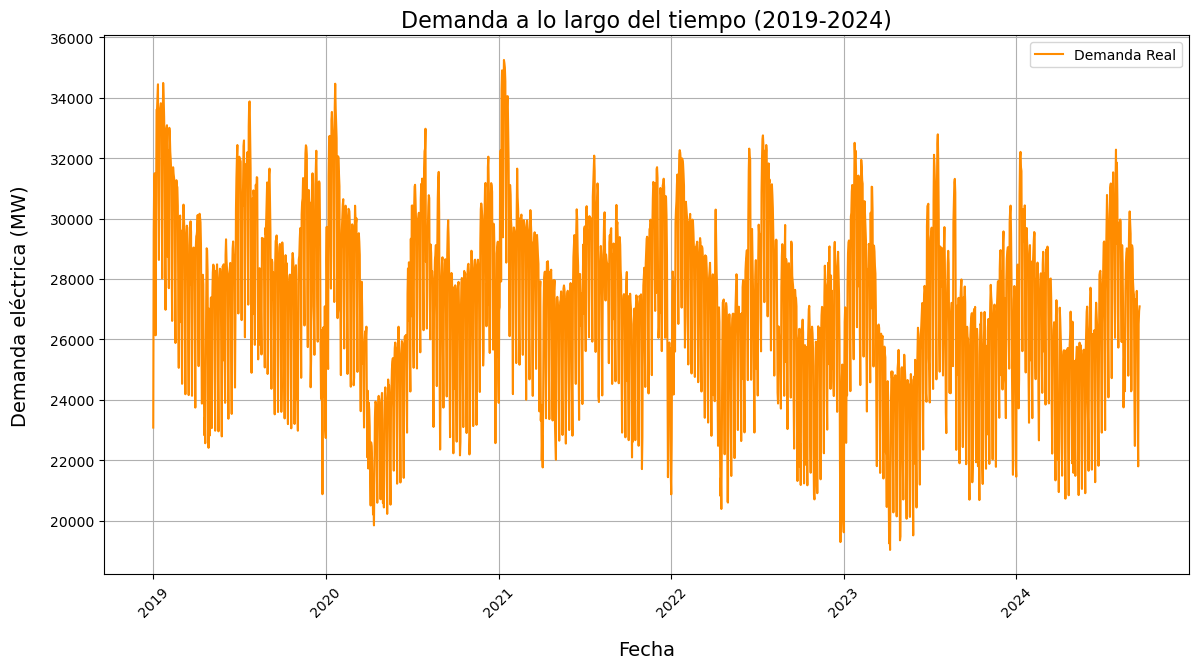
\includegraphics[width=0.9\textwidth]{Images/tfm-3.4A.png}
    \caption{Representación de la demanda eléctrica a lo largo del tiempo (Elaboración propia)}
    \label{fig:demanda_tiempo}
\end{figure}

La Figura \ref{fig:demanda_tiempo} muestra la demanda eléctrica a lo largo del tiempo, donde se pueden identificar patrones estacionales anuales. Se observan fuertes variaciones entre los cambios de trimestre, destacando especialmente al inicio de cada año. El gráfico no es una simple línea, sino que presenta un grosor que refleja las grandes variaciones diarias. A simple vista, se distinguen patrones anuales, trimestrales y diarios. También son interesantes las representaciones temporales de las variables exógenas, en este caso, la temperatura (Figura \ref{fig:temperatura_tiempo}) y la humedad relativa (Figura \ref{fig:humedad_tiempo}), ya que el resto no proporciona información adicional.

\begin{figure}[H]
    \centering
    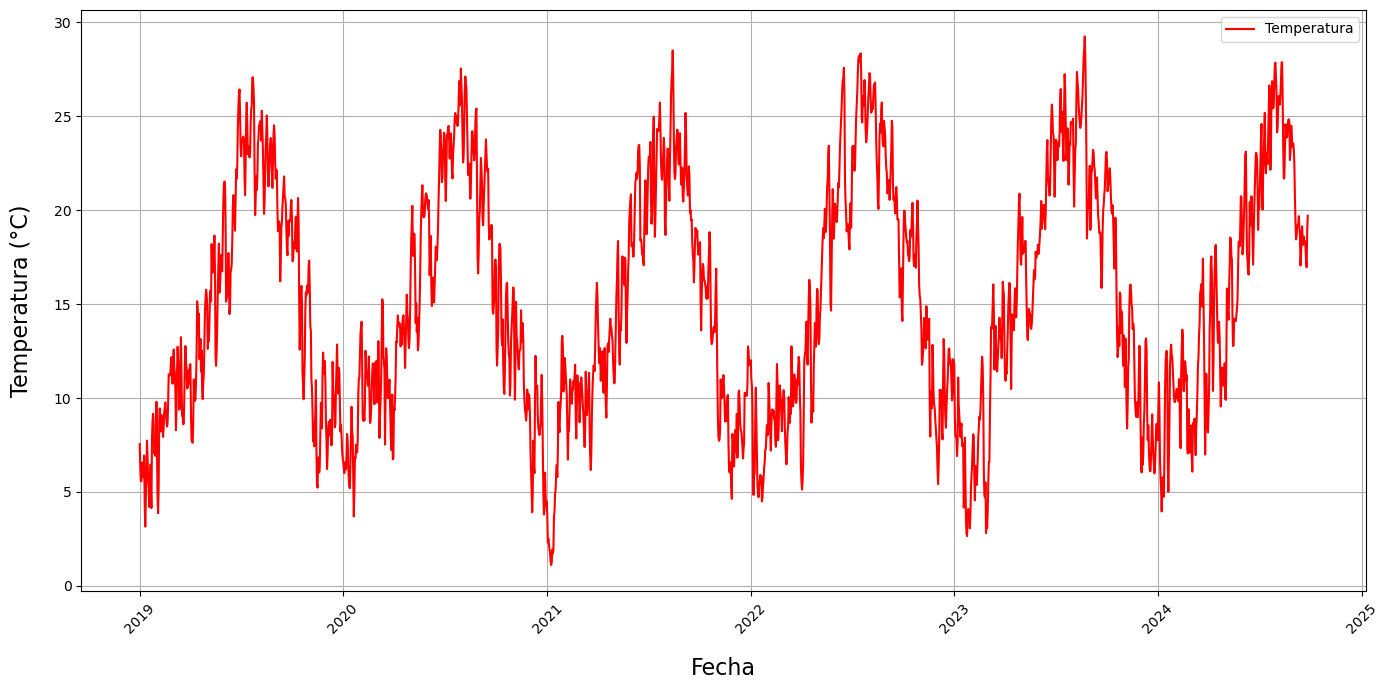
\includegraphics[width=0.9\textwidth]{Images/tfm-3.4B.png}
    \caption{Representación de la temperatura a lo largo del tiempo (Elaboración propia)}
    \label{fig:temperatura_tiempo}
\end{figure}

\begin{figure}[H]
    \centering
    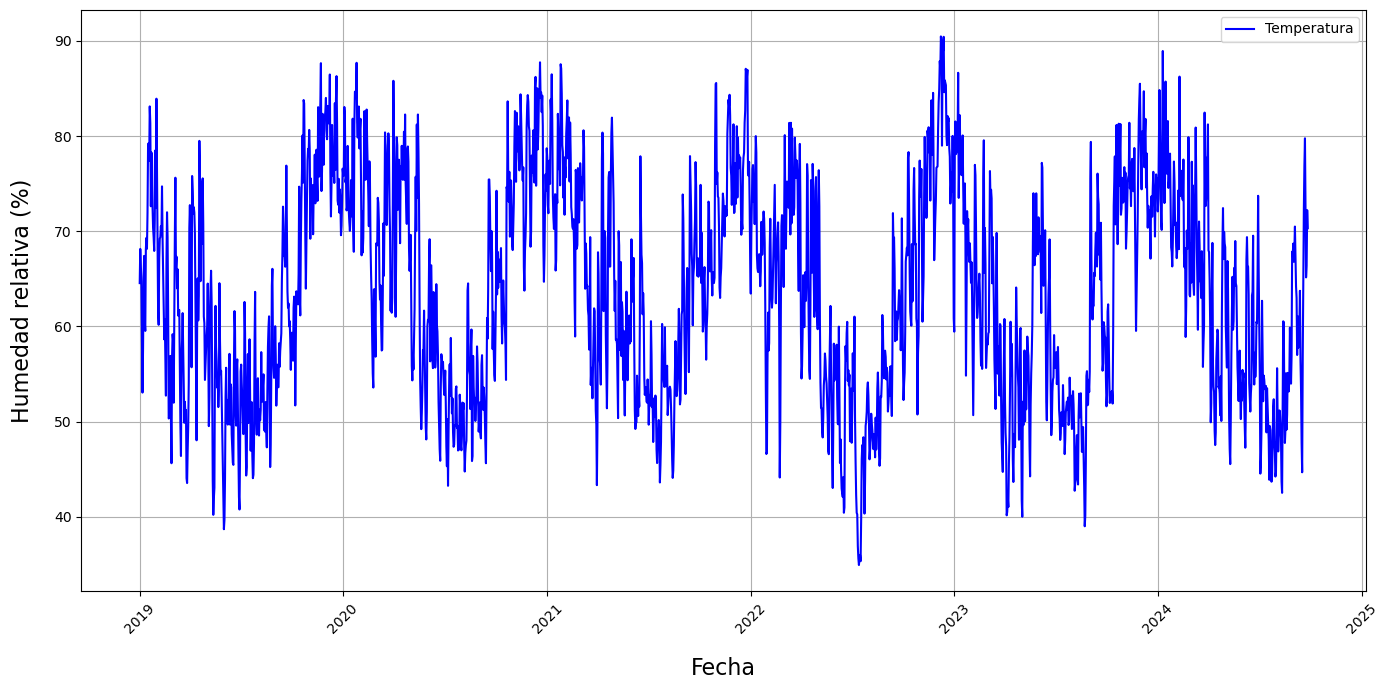
\includegraphics[width=0.9\textwidth]{Images/tfm-3.4C.png}
    \caption{Representación de la humedad relativa a lo largo del tiempo (Elaboración propia)}
    \label{fig:humedad_tiempo}
\end{figure}

Ambas gráficas presentan patrones similares de forma inversa; es decir, cuando la temperatura alcanza un máximo relativo, la humedad registra un mínimo relativo y viceversa. La temperatura exhibe patrones anuales, con máximos en torno a los meses de julio y agosto, y mínimos al inicio y al final del año. Además, muestra una tendencia creciente a lo largo del tiempo. Por otro lado, la humedad relativa presenta características opuestas, aunque se observan valores más fluctuantes de un día para otro, lo que genera la sensación de mayor ruido.

\subsection{Estadística descriptiva}

Una buena manera de comenzar con el análisis de un conjunto de datos se basa en comprender la estadística descriptiva básica. De esa manera se pueden ver características generales de los datos y posibles patrones. La Tabla \ref{tbl:est_stat} muestra un resumen de las magnitudes estadísticas básicas.


\begin{table}[H]
\centering
\caption{\\ Magnitudes estadísticas básicas}
\renewcommand{\arraystretch}{1.2}
\begin{tabular}{lllllll}
\toprule
\textbf{Magnitud} & \textbf{Demanda} & \textbf{Tmed} & \textbf{Hrmedia} & \textbf{Diasem} & \textbf{Trim} & \textbf{Festivo} \\ \midrule

count   & 2088  & 2088 & 2088  & 2088  & 2088 & 2088 \\  \hline
mean    & 27140,89 & 15,18    & 63,74    & 3,00     & 1,44     & 0,03 \\ \hline
std     & 2959,98  & 6,27     & 11,38    & 2,00     & 1,10     & 0,16 \\ \hline
min     & 19032,36 & 1,11     & 34,94    & 0,00     & 0,00     & 0,00 \\ \hline
25\%    & 25060,64 & 10,00    & 54,12    & 1,00     & 0,00     & 0,00 \\ \hline
50\%    & 27330,14 & 14,44    & 63,62    & 3,00     & 1,00     & 0,00 \\ \hline
75\%    & 29223,67 & 20,50    & 73,22    & 5,00     & 2,00     & 0,00 \\ \hline
max     & 35252,53 & 29,25    & 90,46    & 6,00     & 3,00     & 1,00 \\ 

\bottomrule
\end{tabular}
\label{tbl:est_stat}
\caption*{\textit{Nota}: (Elaboración propia)}
\end{table}


Donde:

\begin{itemize}
    \item \textbf{count}: número de valores no nulos.

    \item \textbf{mean}: media.

    \item \textbf{std}: desviación estándar.

    \item \textbf{min, max}: mínimo y máximo absolutos, respectivamente.

    \item \textbf{25\%, 50\%, 75\%}: primer cuartil, mediana y tercer cuartil, respectivamente.
\end{itemize}

La cantidad de valores de cada una de las variables corresponde con el número total de días que contiene el dataset, confirmando la inexistencia de los valores nulos. La gran similitud entre la media y la mediana sugiere que no hay una dispersión considerable en ninguna de las variables estudiadas. La media y la mediana permiten, además, crear una idea de que valores son los más comunes o de referencia en el conjunto de datos. El valor de la media de la variable \textit{trim} debería de ser 1.5 en el caso que se estuviese trabajando con valores completos, en este caso no se han considerado los últimos 100 días del año 2024.

Estas son una de las muchas interpretaciones que se pueden hacer simplemente conociendo las magnitudes estadísticas básicas. Otra información de valor esta relacionada con la distribución de las variables. Para ello se representan los histogramas de la variable objetivo y de las variables exógenas climáticas.

\begin{figure}[H]
    \centering
    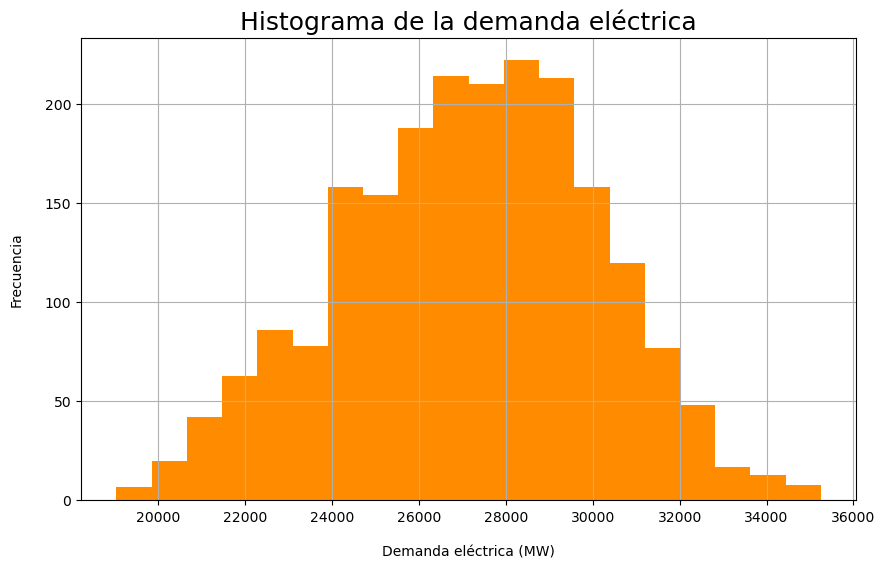
\includegraphics[width=0.75\textwidth]{Images/tfm-3.1A.png}
    \caption{Distribución de la demanda eléctrica (Elaboración propia)}
    \label{fig:hist_demanda}
\end{figure}

\begin{figure}[H]
    \centering
    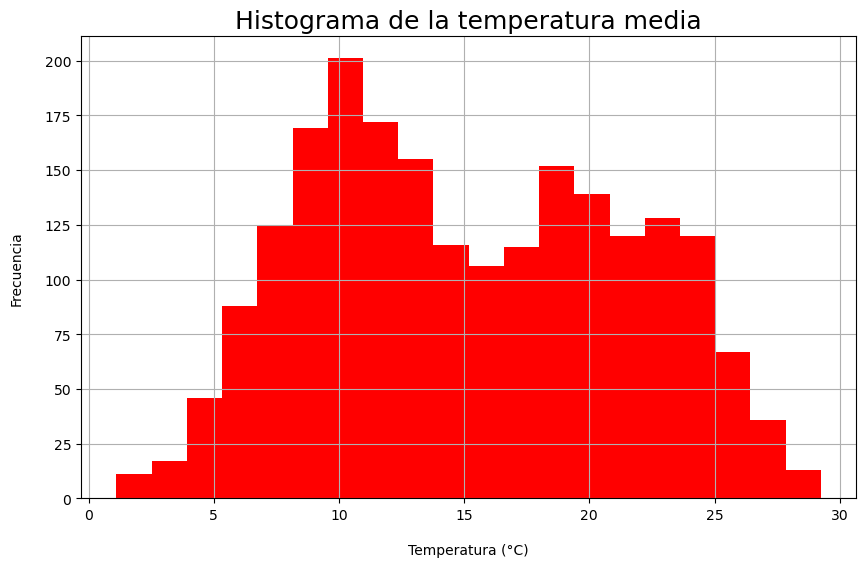
\includegraphics[width=0.75\textwidth]{Images/tfm-3.1B.png}
    \caption{Distribución de la temperatura (Elaboración propia)}
    \label{fig:hist_temp}
\end{figure}

\begin{figure}[H]
    \centering
    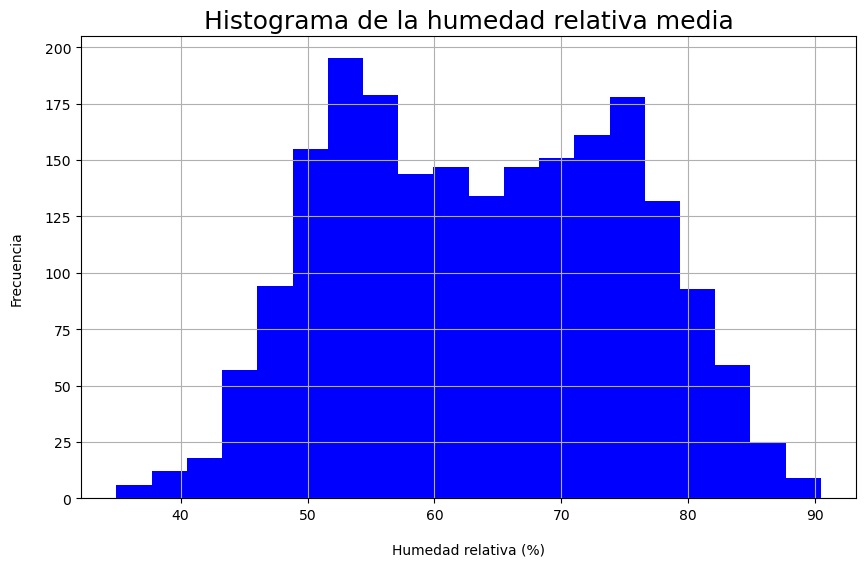
\includegraphics[width=0.75\textwidth]{Images/tfm-3.1C.png}
    \caption{Distribución de la humedad relativa (Elaboración propia)}
    \label{fig:hist_humedad}
\end{figure}

El histograma de la demanda eléctrica (Figura \ref{fig:hist_demanda}) muestra una forma similar a una distribución normal. En contraste, las variables exógenas (Figuras \ref{fig:hist_temp} y \ref{fig:hist_humedad}) presentan la existencia de dos máximos relativos, lo que sugiere que sus distribuciones podrían ser mezclas de gaussianas o distribuciones bimodales. Este hallazgo es relevante para conocer las características básicas de los datos y entender los posibles resultados en algunos modelos de predicción. 

\subsection{Correlación entre variables. Pearson}

Antes de nutrir a los modelos, es fundamental conocer la correlación existente entre el conjunto de variables que conforman el dataset. La existencia de variables altamente relacionadas entre sí puede causar redundancia o repetición de la información inherente en los datos, lo que puede empeorar los resultados de los algoritmos entrenados. La forma tradicional de conocer la correlación entre variables se basa en el índice de correlación de Pearson, el cual es una medida estadística que evalúa la fuerza y la dirección de la relación lineal entre dos variables cuantitativas. La matriz de correlaciones (Figura \ref{fig:mat_corr}) representa cada uno de los índices de Pearson por pares.

En primera instancia, se debe enfocar el análisis de la matriz de correlaciones en aquellas relaciones que involucren la variable objetivo. La única relación a considerar con la demanda eléctrica es la del día de la semana, seguida de los días festivos. El resto de las relaciones tienen valores tan bajos que no deben ser tenidos en cuenta. Dado que el índice de correlación de Pearson solo captura relaciones lineales entre variables, esto sugiere que la naturaleza de los datos es más compleja que una simple relación lineal. Sin embargo, en las relaciones con el resto de las variables, sí aparecen valores más altos, como en el caso de la temperatura con el trimestre y la temperatura con la humedad relativa.

\begin{figure}[H]
    \centering
    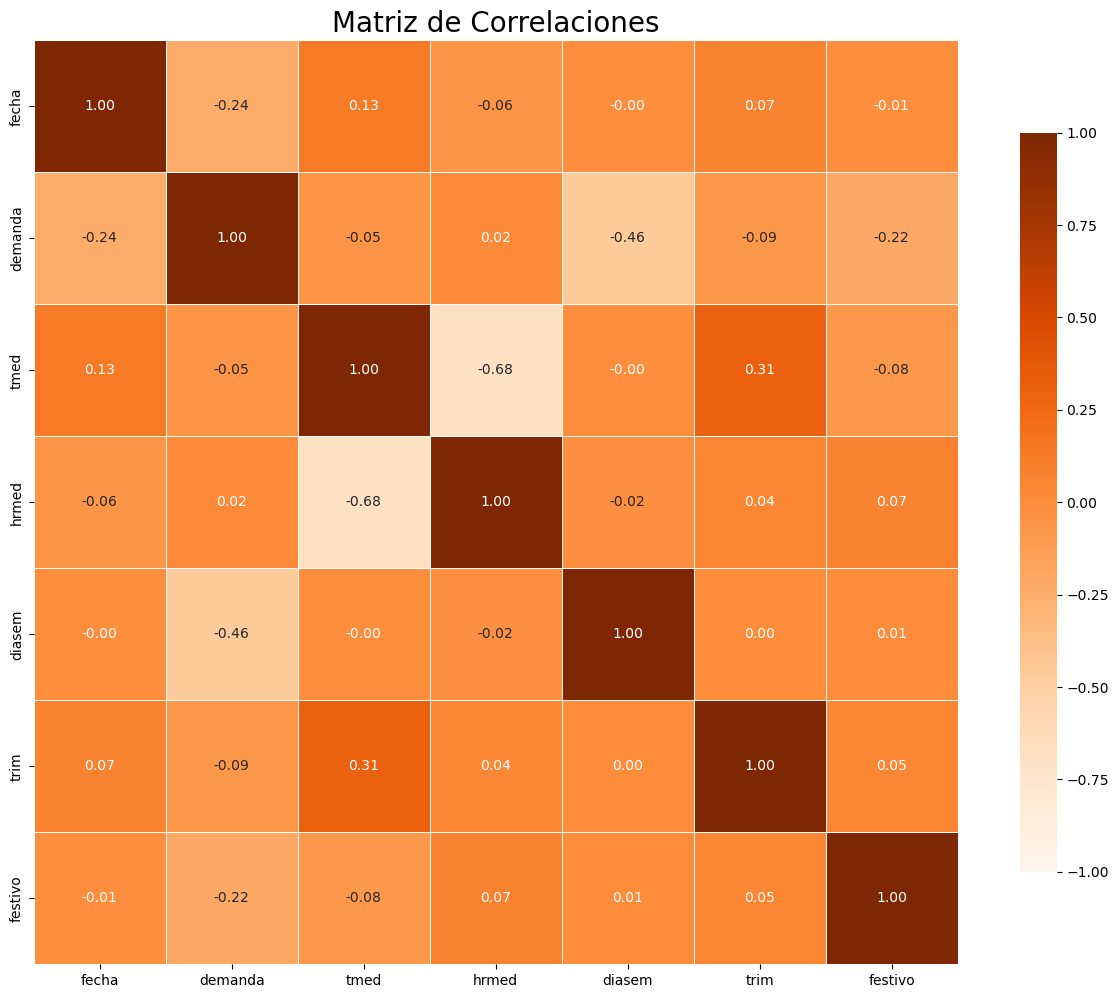
\includegraphics[width=1\textwidth]{Images/tfm-3.3.png}
    \caption{Correlación entre variables con índice de correlación de Pearson (Elaboración propia)}
    \label{fig:mat_corr}
\end{figure}



\subsection{Dispersión de los datos}

Dado que la matriz de correlaciones no ha proporcionado resultados suficientemente positivos, es necesario seguir otra estrategia para comprender mejor las relaciones entre las variables. Una buena opción es representar gráficos de dispersión por pares, ya que pueden aportar información adicional al análisis del conjunto de datos.

\begin{figure}[H]
    \centering
    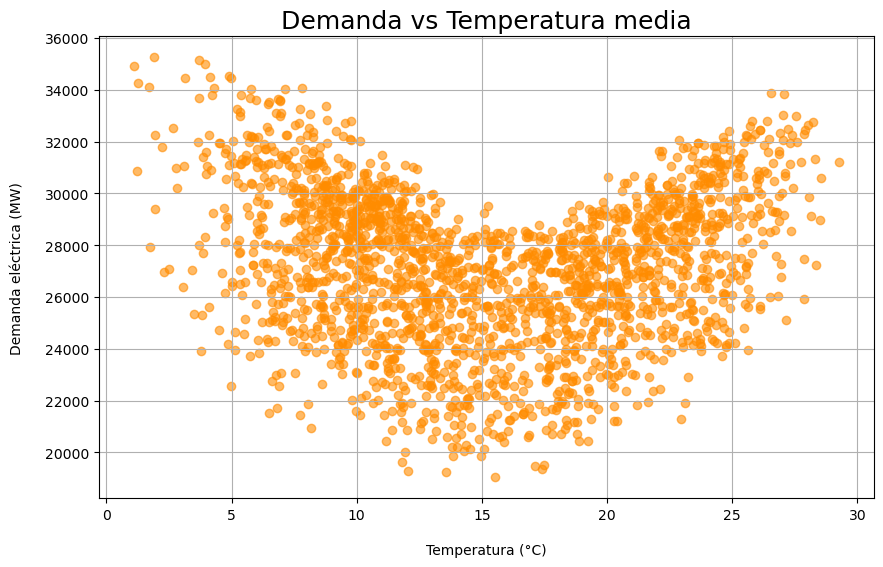
\includegraphics[width=0.9\textwidth]{Images/tfm-3.2A.png}
    \caption{Gráfico de dispersión de la demanda y la temperatura (Elaboración propia)}
    \label{fig:demvstemp}
\end{figure}

\begin{figure}[H]
    \centering
    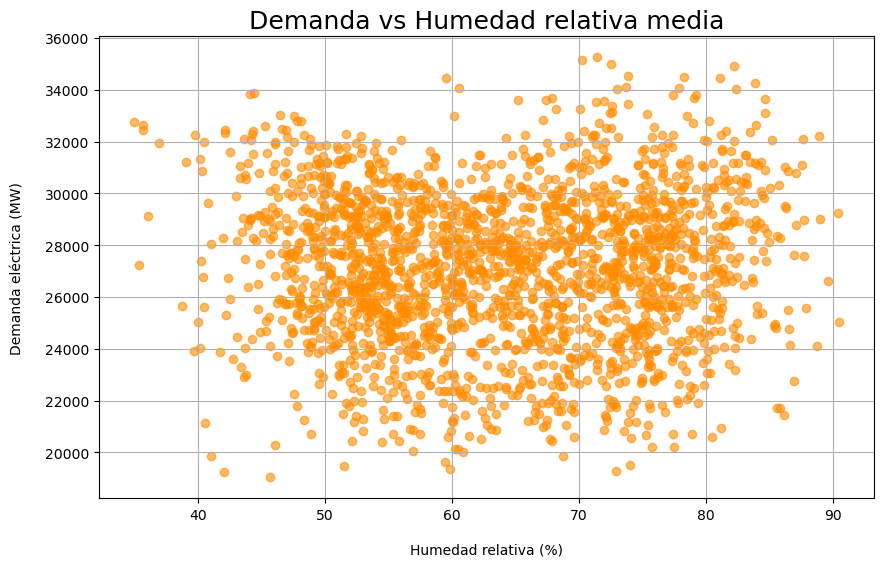
\includegraphics[width=0.9\textwidth]{Images/tfm-3.2B.png}
    \caption{Gráfico de dispersión de la demanda y la humedad relativa (Elaboración propia)}
    \label{fig:demvshum}
\end{figure}

\begin{figure}[H]
    \centering
    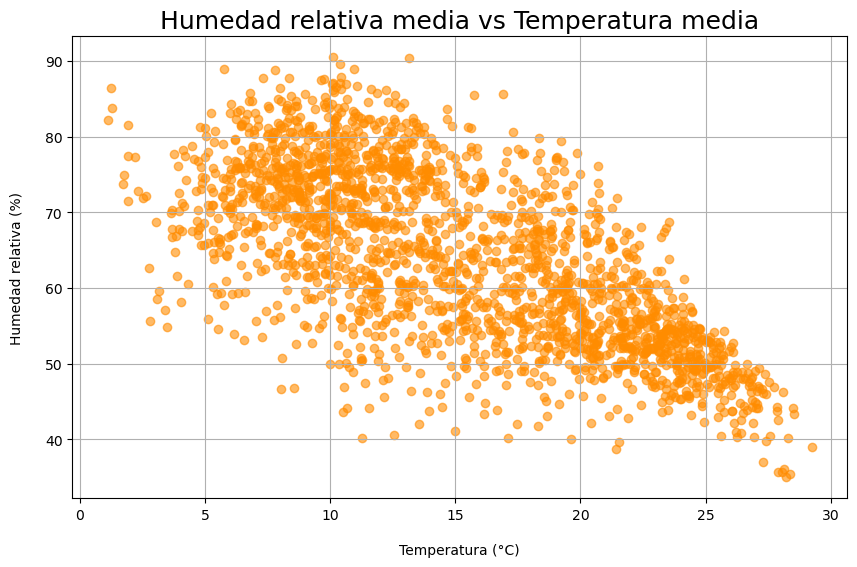
\includegraphics[width=0.9\textwidth]{Images/tfm-3.2C.png}
    \caption{Gráfico de dispersión de la humedad relativa y de la temperatura (Elaboración propia)}
    \label{fig:humvstemp}
\end{figure}

Estos diagramas ofrecen pistas sobre la posible correlación entre las variables representadas. Se observa un patrón entre la demanda eléctrica y la temperatura que sugiere la existencia de una relación no lineal entre ambas variables (Figura \ref{fig:demvstemp}). En cambio, no se aprecia un patrón definido entre la demanda y la humedad relativa, donde solo se observa una nube de puntos (Figura \ref{fig:demvshum}). Además, como era de esperar, el patrón en la dispersión de la temperatura y la humedad relativa muestra una relación de proporcionalidad inversa, es decir, una relación lineal con pendiente negativa (Figura \ref{fig:humvstemp}).

Para el análisis del resto de variables, variables exógenas temporales en este caso, se usan los diagramas de caja (boxplot). Este tipo de gráfico permite identificar rápidamente la mediana, los cuartiles y los valores atípicos. El primer y tercer cuartil están delimitados por una figura rectangular, definida como caja.

En la Figura \ref{fig:BX_trim}, que representa la demanda eléctrica por trimestres, se pueden observar ciertos patrones estacionales a nivel trimestral. La variabilidad de los datos no es muy pronunciada y no se detecta un número significativo de valores atípicos. En los trimestres 1 y 3, la demanda es mayor en comparación con el resto.

\begin{figure}[H]
    \centering
    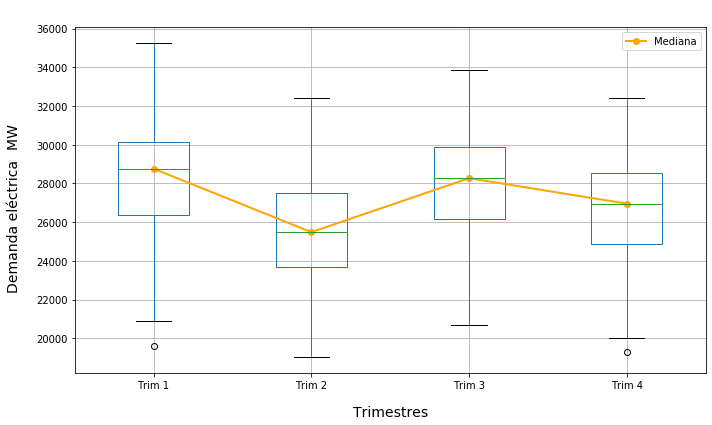
\includegraphics[width=0.9\textwidth]{Images/tfm-3.5A.png}
    \caption{Boxplot de la demanda por trimestres (Elaboración propia)}
    \label{fig:BX_trim}
\end{figure}

Por otro lado, la Figura \ref{fig:BX_sem} muestra el diagrama de caja de la demanda eléctrica por días de la semana. En esta gráfica, hay una mayor cantidad de valores atípicos en comparación con la anterior, especialmente en los miércoles y viernes. La demanda presenta un ligero aumento de lunes a miércoles, mientras que, a partir del jueves hasta el domingo, disminuye, destacándose caídas significativas durante los días del fin de semana.


\begin{figure}[H]
    \centering
    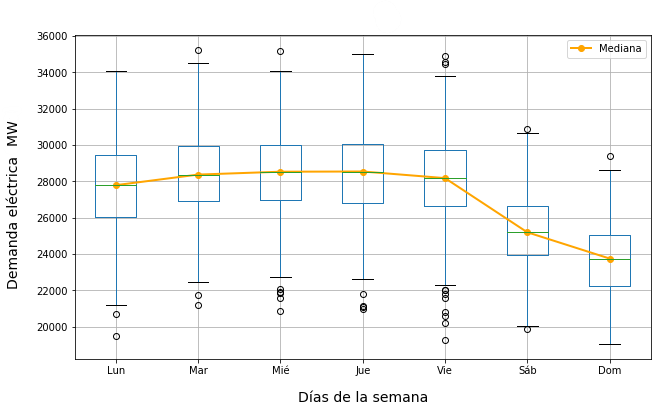
\includegraphics[width=0.9\textwidth]{Images/tfm-3.5B.png}
    \caption{Boxplot de la demanda por días de la semana (Elaboración propia)}
    \label{fig:BX_sem}
\end{figure}

Finalmente, se debe mencionar la influencia de los días festivos en la demanda eléctrica. La Figura \ref{fig:BX_festivos} presenta un boxplot que revela una gran diferencia entre los días festivos y los no festivos, siendo la demanda eléctrica significativamente menor en estos últimos.

\begin{figure}[H]
    \centering
    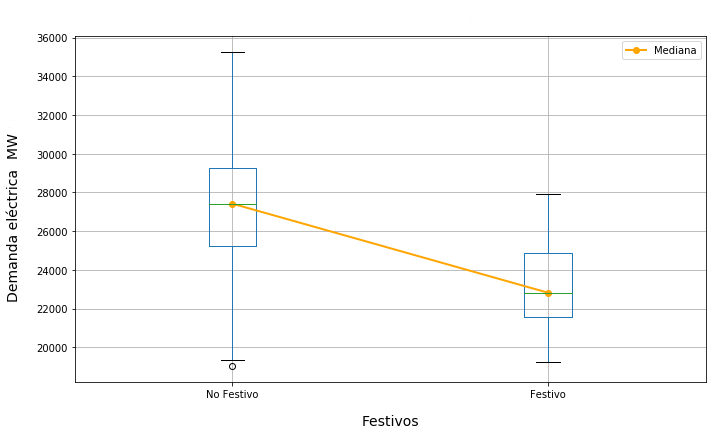
\includegraphics[width=0.9\textwidth]{Images/tfm-3.5C.png}
    \caption{Boxplot de la demanda por días festivos (Elaboración propia)}
    \label{fig:BX_festivos}
\end{figure}




\subsection{Análisis de la serie temporal}

En el tipo de problema que involucra este proyecto, es fundamental conocer las características básicas de la serie temporal asociada a la variable objetivo. En primera instancia, se descompone la serie temporal utilizando un modelo aditivo. Debido a que el análisis de la totalidad de los datos dificultaba la observación de patrones, se ha optado por seleccionar un año aleatorio; en este caso, el 2022.

La Figura \ref{fig:desc_2022} representa gráficamente cada una de las componentes de la serie temporal, de las cuales se pueden extraer las siguientes conclusiones: la tendencia no es lineal y presenta etapas de descenso en el primer y segundo trimestre, tal como se había analizado en los diagramas de caja. La estacionalidad indica patrones principalmente semanales, lo que podría sugerir el número de lags adecuado a utilizar en los modelos. La parte residual muestra picos más altos, especialmente a nivel mensual.

\begin{figure}[H]
    \centering
    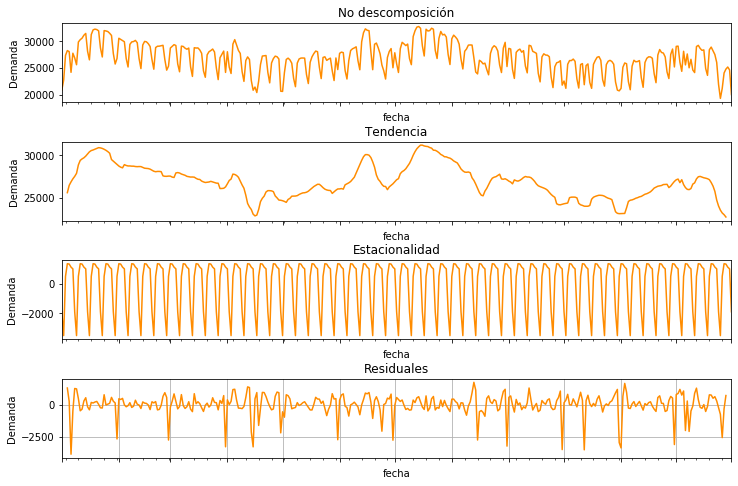
\includegraphics[width=0.95\textwidth]{Images/tfm-3.6.png}
    \caption{Descomposición de la serie temporal de la demanda del año 2022 (Elaboración propia)}
    \label{fig:desc_2022}
\end{figure}



Para confirmar el número óptimo de lags, se utilizan la autocorrelación (Figura \ref{fig:autoc}) y la autocorrelación parcial (Figura \ref{fig:autocp}). Tanto la autocorrelación como la autocorrelación parcial sugieren elegir el número de lags como 7, exceptuando el caso de 2 en el segundo análisis, cuya elección carece de sentido.

\begin{figure}[H]
    \centering
    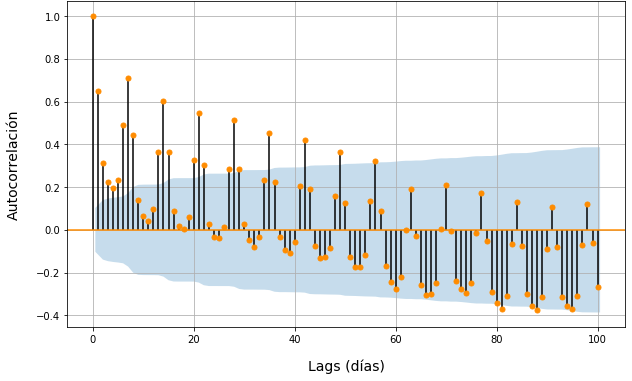
\includegraphics[width=0.95\textwidth]{Images/tfm-3.7A.png}
    \caption{Representación gráfica de la autocorrelación (Elaboración propia)}
    \label{fig:autoc}
\end{figure}

\begin{figure}[H]
    \centering
    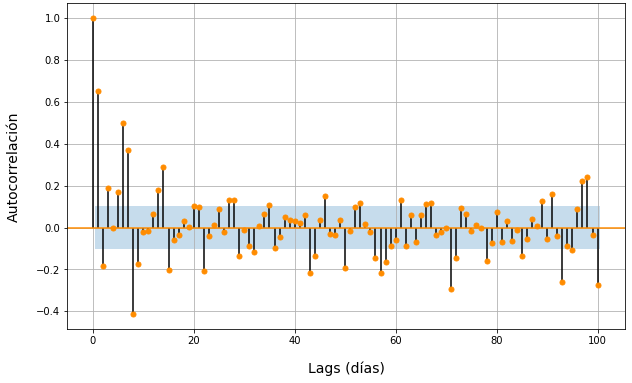
\includegraphics[width=0.95\textwidth]{Images/tfm-3.7B.png}
    \caption{Representación gráfica de la autocorrelación parcial (Elaboración propia)}
    \label{fig:autocp}
\end{figure}

\section{Entrenamiento de los modelos}

A continuación, se describe la metodología seguida para el entrenamiento de los modelos seleccionados para la predicción de la demanda eléctrica. Se busca una elección diversa de algoritmos para estudiar diferentes comportamientos, manteniendo escenarios lo más similares posibles entre cada uno. Los modelos a entrenar son: ARIMA-ARIMAX, Decision Tree, Random Forest, XGBoost y LSTM. Para el entrenamiento, se dividió el conjunto de datos en un subconjunto de entrenamiento (80$\%$ de los datos, desde el 01/01/2019 hasta el 05/08/2023) y un subconjunto de prueba o test (20$\%$ restante, desde el 05/08/2023 hasta el 26/09/2024).

Para cada modelo, se selecciona un conjunto de hiperparámetros a explorar mediante dos técnicas de optimización: Grid Search y optimización bayesiana. La primera alternativa se aplica en los modelos más tradicionales, como ARIMA-ARIMAX, y en el modelo de aprendizaje profundo, LSTM; mientras que, para el resto de modelos de Machine Learning, se emplea la optimización bayesiana.

Para la validación de los modelos, se utiliza un proceso de backtesting sin reajuste, escogido debido a los altos requerimientos computacionales asociados con otras técnicas de backtesting, que no mostraron mejoras significativas en los resultados en comparación con la metodología seleccionada. Para evitar el sobreajuste (overfitting), se controla el espacio de hiperparámetros de cada modelo, limitando el ajuste a valores que no incrementaran excesivamente la complejidad. También se seleccionan cuidadosamente las mejores variables exógenas, restringiendo su número para prevenir excesos. La métrica escogida ha sido el MAE, por su robustez frente a los outliers, que no se han considerado tan relevantes, y por su facilidad de interpretación.

En cada iteración, el conjunto de entrenamiento predijo únicamente un valor a futuro. Esta estrategia mejora significativamente la precisión de los resultados, aunque implica un mayor costo computacional, que se considera asumible en este contexto. Con base en los resultados de la autocorrelación y la autocorrelación parcial, se ha seleccionado un número de lags igual a 7.

La librería principal utilizada, y que ha sido de gran utilidad en la aplicación de modelos para series temporales, es \textit{skforecast} (\cite{skforecast}). Su característica más destacada es su enfoque en el forecasting mediante regresores, aplicando el método autoregresivo en el cual se predicen valores futuros en función de valores pasados de la serie temporal. Esta librería simplifica la conversión de problemas de series temporales a problemas supervisados, transformando los datos de la serie en conjuntos de características y etiquetas adecuados para el entrenamiento de modelos de predicción.


\subsection{Modelo ARIMA-ARIMAX}

El primer modelo entrenado corresponde a la categoría comúnmente denotada como modelos tradicionales. Este se trata del único algoritmo no perteneciente al ámbito del Machine Learning en este proyecto. Sirve para establecer las bases de los resultados y permitir una mejor comparación con el resto de técnicas.

Para poder aplicar este modelo, se ha tenido que hacer un análisis previo de la estacionariedad de la serie temporal. Se ha aplicado la prueba ADF, usando el criterio AIC para seleccionar el número de lags. El AIC es una medida que se usa para comparar modelos estadísticos, basándose en la idea de se debe proporcionar un buen ajuste a los datos sin ser un modelo excesivamente complejo. Los resultados han sido:

\begin{itemize}
    \item Estadístico ADF: -5.05.
    \item Valor \textit{p}: 1.75 $\times$ 10$^{-5}$.
    \item Valores críticos: 1$\%$: -3.43; 5$\%$: -2.86; 10$\%$: -2.57.
\end{itemize}

Como el estadístico ADF es significativamente más negativo que los valores críticos y el valor \textit{p} es aproximadamente nulo, existe la suficiente evidencia para rechazar la hipótesis nula. De esta manera se puede afirmar que la serie temporal es estacionaria, pudiendo aplicar los modelos ARIMA y ARIMAX sin tratamientos adicionales. Para el entrenamiento del modelo, se ha usado las clase \textit{ForecasterSarimax} y \textit{backtesting$\_$sarimax} de \textit{Skforecast}. De esta manera se ha podido hacer una búsqueda por el espacio de hiperparámetros conformados por \textit{p}, \textit{d} y \textit{q} mediante la técnica Grid Search. 

\subsection{Modelo Decision Tree}

El modelo Decision Tree constituye la estructura fundamental sobre la que se construyen otros modelos más complejos, como el Random Forest y el XGBoost. Esta relación ha facilitado un enfoque común entre estas tres técnicas seleccionadas, aunque cada una difiere en su espacio de hiperparámetros. A continuación, se detalla la metodología empleada para el entrenamiento del árbol de decisión, teniendo en cuenta que el proceso será prácticamente el mismo para los otros dos modelos. 

Para poder usar la técnica basada en el forecaster autoregresivo, se ha usado la clase \textit{ForecasterAutoreg} junto al regresor \textit{DecisionTreeRegressor} de la librería \textit{skforecast}. Posteriormente se ha llevado a cabo la optimización de los hiperparámetros del modelo usando la técnica de optimización bayesiana. El conjunto de hiperparámetros escogido ha sido: \textit{maximum depht}, \textit{maximum branch}, \textit{leaf size} y \textit{split size}. El número de iteraciones escogido ha sido el suficiente para extraer unas predicciones lo suficientemente satisfactorias, pero sin usar altos tiempos en el procesamiento. Una vez escogido el mejor resultado, se usa la clase \textit{backtesting$\_$forecaster} para emplear el proceso de backesting.

\subsection{Modelo Random Forest}

La metodología seguida, tal y como se ha mencionado anteriormente, es similar a la del modelo Decision Tree. Únicamente cambia el regresor escogido, \textit{RandomForestRegressor} y el conjunto de hiperparámetros: \textit{number of estimators}, \textit{maximum samples}, \textit{maximum depth}, \textit{maximum branches}, \textit{leaf size} y \textit{split size}. 

\subsection{Modelo XGBoost}

El entrenamiento ha sido similar al de los dos modelos anteriores. Únicamente cambia el regresor elegido, \textit{RandomForestRegressor} y el conjunto de hiperparámetros: \textit{number of estimators}, \textit{learning rate}, \textit{gamma}, \textit{alpha}, \textit{lambda}, \textit{subsample ratio of the training instances} y \textit{subsample ratio of columns when constructing each tree}.. 

\subsection{Modelo LSTM}

El modelo seleccionado para representar las técnicas de Deep Learning es una red neuronal recurrente (RNN), en específico el modelo LSTM. Debido a la cantidad limitada de datos, se ha escogido una estructura de red neuronal lo más simple posible, conformada por:

\begin{enumerate}
    \item \textbf{Capa de entrada}: la red recibe una serie temporal como entrada. En este paso se establece el número de lags y la cantidad de valores a predecir, es decir, el número de steps.

    \item \textbf{Capa recurrente}: capa de procesamiento LSTM. Contiene un número de unidades recurrentes que se encargan de procesar la secuencia de entrada, manteniendo un estado interno que le permite recordar información importante de pasos anteriores de la serie.

    \item \textbf{Capa densa}: transforma la salida de la capa recurrente en una estructura adecuada para generar las predicciones. Esta función es realizada por las unidades densas, que forman un conjunto de neuronas conectadas. Cada neurona recibe entradas de todas las neuronas de la capa anterior y aplica una suma ponderada seguida de una función de activación para producir una salida.
    
    \item \textbf{Capa de salida}: salida final de la red, ajustada para proporcionar las predicciones finales del entrenamiento del modelo.

    \item \textbf{Optimización y evaluación}: la red utiliza el optimizador Adam para mejorar la convergencia del modelo, ajustando la tasa de aprendizaje de manera adaptativa. La precisión se evalúa mediante la función de pérdida MSE, elegida por su alta sensibilidad a los outliers, lo que permite detectar comportamientos anómalos en el modelo.
\end{enumerate}



El modelo se compila utilizando la clase \textit{create\_and\_compile\_model} de \textit{skforecast}, donde se selecciona el tipo de red LSTM. Este modelo se introduce como regresor en la clase \textit{ForecasterRnn}, que actúa como un forecaster autoregresivo. Es importante que la serie temporal esté normalizada para que el modelo se ajuste correctamente. Además, se ajustan tanto el número de épocas como el tamaño de las muestras utilizadas en cada iteración. Finalmente, para el proceso de backtesting, se utiliza la clase \textit{backtesting\_forecaster\_multiseries}, todas pertenecientes al módulo de \textit{skforecast}.

Para el proceso de optimización del modelo, se ha usado un método simple de Grid Search, que ha buscado en un espacio reducido de los siguientes hiperparámetros: \textit{number of recurrent units}, \textit{number of dense units}, \textit{learning rate}, \textit{number of epochs} y \textit{batch size}. El resto se han mantenido fijos. 

El sobreajuste del modelo se ha controlado mediante el análisis de la gráfica de entrenamiento versus validación. Para ello se ha reservado una pequeña parte de los datos para hacer la validación, comprendida desde el 01/01/2023 hasta el 05/08/2023 (inicio del conjunto de entrenamiento). En este análisis, si la pérdida de entrenamiento sigue disminuyendo mientras que la pérdida de validación comienza a aumentar, esto indica que el modelo está aprendiendo patrones específicos de los datos de entrenamiento sin generalizar adecuadamente a nuevos datos. Además, una diferencia notable entre las curvas de pérdida de entrenamiento y validación a lo largo de las épocas sugiere que el modelo ha ajustado demasiado sus parámetros a los datos de entrenamiento, comprometiendo su capacidad de generalización.

\newpage
\chapter{Resultados}\label{cap:cap5}

Una vez entrenados los modelos, es el momento de hacer un análisis adecuado de los resultados para poder extraer conclusiones de valor. Para ello, se van a exponer una serie de tablas que muestren diferentes resultados de cada uno de los modelos, siguiendo un mismo formato. La Tabla \ref{tab:tabla_gen} representa este formato mencionado:

\begin{table}[H]
\centering
\caption{\\ Tabla genérica para la comparación de resultados}
\renewcommand{\arraystretch}{1.5}
\scriptsize
\begin{tabular}{m{1cm} m{1.2cm} m{1.2cm} m{1cm} m{1cm} m{1.2cm} m{1.2cm} m{3.5cm}} 
\toprule
\textbf{Modelo} & \textbf{V. exóg.} & \textbf{Optim.} & \textbf{t (s)} & \textbf{it} & \textbf{t/it (s)} & \textbf{MAE} & \textbf{Hiperparámetros} \\
\midrule
modelo & Grupo 0 & - & - & - & - & - & - \\[0.5em]
\hline
modelo & Grupo 1 & - & - & - & - & - & - \\[0.5em]
\hline
modelo & Grupo 2 & - & - & - & - & - & - \\[0.5em]
\hline
modelo & Grupo 3 & - & - & - & - & - & - \\[0.5em]
\hline
modelo & Grupo 4 & - & - & - & - & - & - \\[0.5em]
\hline
modelo & Grupo 5 & - & - & - & - & - & - \\
\bottomrule
\end{tabular}
\label{tab:tabla_gen}
\caption*{\textit{Nota}: (Elaboración propia)}
\end{table}


Donde cada una de las columnas es:

\begin{itemize}
    \item \textbf{Modelo}: modelo escogido.

    \item \textbf{V. exóg.}: grupo de variables exógenas.
    \begin{itemize}
        \item Grupo 0: sin variables exógenas.
        \item Grupo 1: diasem.
        \item Grupo 2: diasem, trim.
        \item Grupo 3: diasem, trim, festivo.
        \item Grupo 4: diasem, trim, festivo, tmed.
        \item Grupo 5: diasem, trim, festivo, tmed, hrmed.
    \end{itemize}

    \item \textbf{Optim.}: ténnica de optimización usada.

    \item \textbf{t (s)}: tiempo total que ha tarado el programa en ejecutarse en segundos.

    \item \textbf{it}: número de iteraciones empleadas por el programa.

    \item \textbf{t/it (s)}: tiempo por iteración en segundos.

    \item \textbf{MAE}: valor de la métrica del mejor resultado.

    \item \textbf{Hiperparámetros}: valor de los hiperparámetros del mejor resultado.
\end{itemize}

\section{Comparativa de los resultados por modelo}

En esta sección se van a analizar los resultados individuales de cada modelo. Para ello se va a seguir una sencilla metodología basada en el siguiente esquema:

\begin{enumerate}
    \item \textbf{Tabla comparativa}: se muestra la comparación de los resultados para cada uno de los grupos de las variables exógenas. Se sigue el formato de la tabla genérica antes mencionada.

    \item \textbf{Análisis}: desarrollo del análisis en forma de texto. Donde se comienzan a extraer las primeras conclusiones del proyecto.

    \item \textbf{Representación gráfica}: representación gráfica de los valores predichos vs los valores reales del grupo de variables exógenas con mejores resultados.

    \item \textbf{Descripción de la gráfica y conclusiones}: pequeño parrafo aclaratorio. 
\end{enumerate}

\subsection{Modelo ARIMA-ARIMAX}

\begin{table}[H]
\centering
\caption{\\ Resultados de la optimización de los modelos ARIMA-ARIMAX}
\scriptsize
\begin{tabular}{m{1cm} m{1.2cm} m{1.2cm} m{1cm} m{1cm} m{1.2cm} m{1.2cm} m{2cm}} 
\toprule
\textbf{Modelo} & \textbf{V. exóg.} & \textbf{Optim.} & \textbf{t (s)} & \textbf{it} & \textbf{t/it (s)} & \textbf{MAE} & \textbf{Hiperparámetros} \\
\midrule
ARIMA   & Grupo 0 & Grid Search & 532,09 & 27 & 19,71 & 1311,67 & \texttt{$p=2$ \newline $d=1$ \newline $q=3$} \\[0.5em]
\hline
ARIMAX  & Grupo 1 & Grid Search & 317,42 & 27 & 11,76 & 861,65 & \texttt{$p=2$ \newline $d=1$ \newline $q=3$} \\[0.5em]
\hline
ARIMAX  & Grupo 2 & Grid Search & 320,08 & 27 & 11,85 & 859,77 & \texttt{$p=2$ \newline $d=1$ \newline $q=3$} \\[0.5em]
\hline
ARIMAX  & Grupo 3 & Grid Search & 322,12 & 27 & 11,93 & 780,22 & \texttt{$p=2$ \newline $d=1$ \newline $q=3$} \\[0.5em]
\hline
ARIMAX  & Grupo 4 & Grid Search & 421,01 & 27 & 15,59 & 778,73 & \texttt{$p=2$ \newline $d=1$ \newline $q=3$} \\[0.5em]
\hline
ARIMAX  & Grupo 5 & Grid Search & 438,50 & 27 & 16,24 & 772,99 & \texttt{$p=2$ \newline $d=1$ \newline $q=3$} \\
\bottomrule
\end{tabular}
\label{tab:resultados_optimizacion_arima}
\caption*{\textit{Nota}:  
los hiperparámetros son \textit{p}, \textit{d} y \textit{q}. (Elaboración propia)}
\end{table}

Para el entrenamiento del modelo ARIMA-ARIMAX se ha aplicado la técnica de optimización de Grid Search en el espacio de hiperparámetros de \textit{p}, \textit{d}, \textit{p}, cada uno variando entre 1 y 3. Este método de optimización ha sido suficiente, ya que el conjunto de hiperparámetros es bastante simple, compuesto únicamente por tres valores, que son números enteros. No se ha optado por aumentar el espacio de observación, ya que los resultados empeoraban y el modelo se volvía cada vez más complejo, incrementando así la probabilidad de sobreajuste.

Se observa que, para todos los grupos, se mantiene el mismo valor de los hiperparámetros después de la optimización: \textit{p} = 2, \textit{d} = 1 y \textit{q} = 3. Esto sugiere que los resultados no dependen de la selección de los hiperparámetros, sino más bien de la influencia de las variables exógenas utilizadas. El peor resultado corresponde al modelo ARIMA (sin variables exógenas), que presenta un MAE muy superior al del modelo entrenado con una variable exógena (Grupo 1). En contraste, el mejor resultado se obtiene con el modelo que contiene las variables exógenas del Grupo 5, con MAE $\approx$ 773, mejorando en casi un 59$\%$ el MAE del modelo con peor desempeño (Grupo 0). 

En cuanto a tiempos de procesamiento, todos los modelos se encuentran en el intervalo de 11 a 20 segundos por iteración. Se observa que el modelo que más recursos ha necesitado ha sido el correspondiente al Grupo 0 de variables exógenas. Esto puede generar confusión, ya que, intuitivamente, se podría pensar que a medida que aumenta el número de variables exógenas, el modelo debería enfrentarse a una mayor complejidad y, por lo tanto, requerir más tiempo para aprender. Cuando se añade la primera variable exógena (Grupo 1), el modelo obtiene información adicional y no se limita únicamente a adaptarse a sus valores pasados. Por lo que la complejidad no siempre se relaciona directamente con el número de variables, ya que la falta de contexto puede dificultar el aprendizaje del modelo. A medida que se añaden más variables exógenas, el proceso de aprendizaje se vuelve cada vez más costoso de manera progresiva, pero sin superar los tiempos de procesamiento observados en el caso del Grupo 0.

\begin{figure}[H]
    \centering
    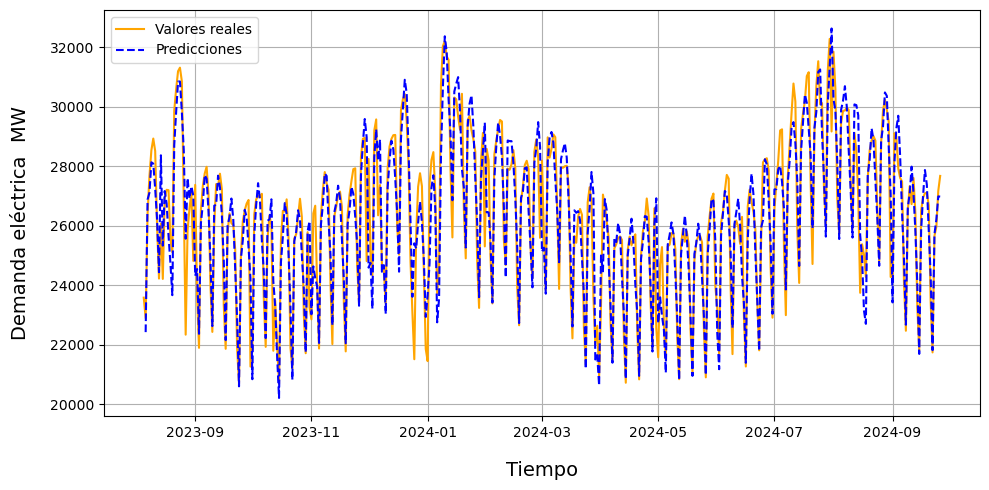
\includegraphics[width=0.9\textwidth]{Images/tfm-4.1(arimax).png}
    \caption{Representación gráfica de los mejores resultados de los modelos ARIMA y ARIMAX (Elaboración propia) }
    \label{fig:figura_ARIMAX}
\end{figure}

La Figura \ref{fig:figura_ARIMAX} muestra la serie temporal de la mejor predicción del modelo ARIMA-ARIMAX (Grupo 5 de variables exógenas) frente a los valores reales. Se observa que, en general, el modelo se adapta de manera aceptable, excepto en algunos picos específicos. Sobre todo, se han obtenido peores resultados en los meses anteriores al inicio del año 2024. Los días festivos, como el Año Nuevo, son más difíciles de predecir, lo que conlleva más errores. Sin embargo, en los picos de demanda durante los fines de semana se han obtenido mejores resultados. En general, este modelo establece las bases para comparar los resultados con los demás modelos a entrenar, lo que permite identificar puntos de fortaleza y áreas de mejora.


\subsection{Modelo Decision Tree}

\begin{table}[H]
\centering
\caption{\\ Resultados de la optimización del modelo Decision Tree}
\scriptsize
\begin{tabular}{m{1cm} m{1.2cm} m{1.2cm} m{1cm} m{1cm} m{1.2cm} m{1.2cm} m{3.5cm}} 
\toprule
\textbf{Modelo} & \textbf{V. exóg.} & \textbf{Optim.} & \textbf{t (s)} & \textbf{it} & \textbf{t/it (s)} & \textbf{MAE} & \textbf{Hiperparámetros} \\
\midrule
Decision Tree   & Grupo 0 & Bayesiana & 132,45 & 200 & 0,76 & 954,94 & \texttt{$max\_depth=11$ \newline $max\_leaf\_nodes = 62$  \newline $min\_samples\_leaf = 8$ \newline $min\_samples\_split = 19 $} \\[0.5em]
\hline
Decision Tree   & Grupo 1 & Bayesiana & 145,72 & 200 & 0,84 & 833,88 & \texttt{$max\_depth=10$ \newline $max\_leaf\_nodes=64$ \newline $min\_samples\_leaf=10$ \newline $min\_samples\_split=12$} \\[0.5em]
\hline
Decision Tree   & Grupo 2 & Bayesiana & 144,30 & 200 & 0,85 & 833,78 & \texttt{$max\_depth=10$ \newline $max\_leaf\_nodes=64$ \newline $min\_samples\_leaf=10$ \newline $min\_samples\_split=12$} \\[0.5em]
\hline
Decision Tree   & Grupo 3 & Bayesiana & 144,31 & 200 & 0,84 & 809,91 & \texttt{$max\_depth=17$ \newline $max\_leaf\_nodes=68$ \newline $min\_samples\_leaf=10$ \newline $min\_samples\_split=8$} \\[0.5em]
\hline
Decision Tree   & Grupo 4 & Bayesiana & 154,40 & 200 & 0,90 & 790,53 & \texttt{$max\_depth=11$ \newline $max\_leaf\_nodes=53$ \newline $min\_samples\_leaf=4$ \newline $min\_samples\_split=17$} \\[0.5em]
\hline
Decision Tree   & Grupo 5 & Bayesiana & 153,13 & 200 & 0,91 & 792,69 & \texttt{$max\_depth=15$ \newline $max\_leaf\_nodes=67$ \newline $min\_samples\_leaf=4$ \newline $min\_samples\_split=16$} \\
\bottomrule
\end{tabular}
\label{tab:resultados_optimizacion}
\caption*{\textit{Nota}: los hiperparámetros son \textit{max\_depth}: maximum depht ; \textit{max\_leaf\_nodes}: maximum branch; \textit{min\_samples\_leaf}: leaf size; \textit{min\_samples\_split}: split size. (Elaboración propia)}
\end{table}

Se ha utilizado el enfoque de optimización bayesiana para encontrar la mejor combinación posible de hiperparámetros. En los primeros intentos, se exploró un espacio más amplio, y en los últimos se ha ido acotando cada vez más. Se ha fijado el número de iteraciones en 200, un número suficientemente alto para obtener buenos resultados, pero que también busca evitar el sobreajuste, un problema común en los modelos de árboles de decisión.

El valor de los hiperparámetros ha ido variando conforme se han ido añadiendo variables exógenas. El mayor salto en la calidad de los resultados se ha visto desde el modelo correspondiente al Grupo 0 hasta el Grupo 1, donde se ha añadido la primera variable exógena, \textit{diasem}. La adición de las variables \textit{trim} y \textit{hrmed} ha empeorado los resultados con respecto al grupo anterior, ya que el modelo no ha sido capaz de captar nuevas relaciones en estos casos e incluso ha registrado cierto ruido. Comprobando los saltos de grupo a grupo, se puede observar que las variables exógenas que han dado una mayor facilidad en el entrenamiento del modelo son: \textit{diasem}, \textit{festivo} y \textit{tmed}.

Los árboles más profundos han sido los correspondientes al Grupo 3 y Grupo 5 (\textit{max\_depth = 17} y \textit{max\_depth = 15}, respectivamente), lo que evidencia que el algoritmo ha necesitado captar relaciones más complejas, aumentando así el riesgo de sobreajuste. El Grupo 4, aunque no ha sido el árbol con menor profundidad, ha presentado los valores más bajos en el resto de los hiperparámetros. Es decir, se trata del modelo menos complejo y, debido al valor del MAE, ha mostrado la mejor adaptación a los datos de entrenamiento.

En cuanto a los tiempos de procesamiento, ningún modelo ha superado el segundo por iteración, cuyo valor ha ido aumentando progresivamente, en términos generales, a medida que se han ido añadiendo variables exógenas. Es decir, el árbol de decisión se ha entrenado de manera muy rápida, mostrando poco impacto por la inclusión de nuevas variables exógenas.

\begin{figure}[H]
    \centering
    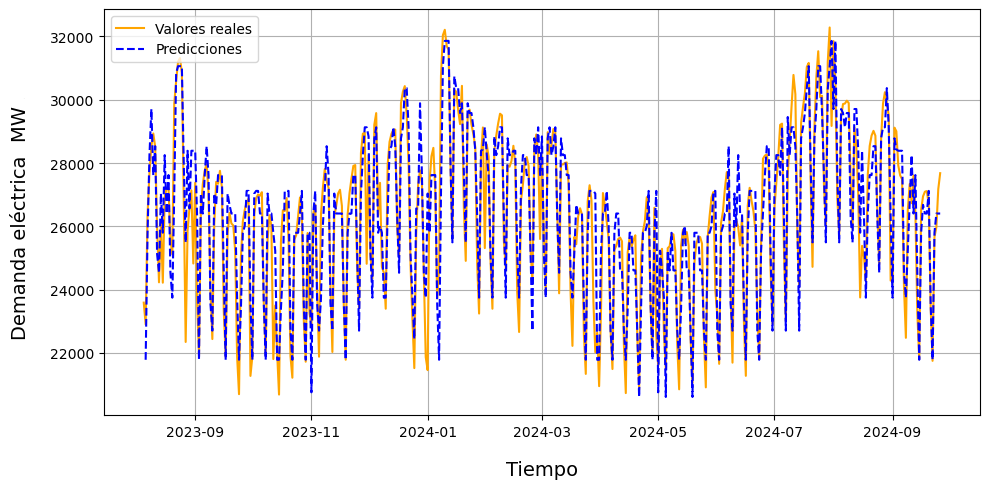
\includegraphics[width=0.9\textwidth]{Images/tfm-4.2(decisiontree).png}
    \caption{Representación gráfica de los mejores resultados del modelo Decision Tree (Elaboración propia) }
    \label{fig:figura_DT}
\end{figure}

La Figura \ref{fig:figura_DT} representa la serie temporal del mejor resultado, correspondiente al Grupo 4 de variables exógenas. En general, el modelo no se ha ajustado adecuadamente a los picos de baja demanda, especialmente los de los domingos. Asimismo, su desempeño en la predicción de días festivos ha sido deficiente, con altas variabilidades observadas en la mayoría de los casos. Sin embargo, el modelo ha mostrado una mejor adaptación a los picos de alta demanda. En términos generales, estas predicciones no reflejan bien la realidad, especialmente en lo que respecta a los picos de baja demanda y a los días festivos.

\subsection{Modelo Random Forest}

\begin{table}[H]
\centering
\caption{\\ Resultados de la optimización del modelo Random Forest}
\scriptsize
\begin{tabular}{m{1cm} m{1.2cm} m{1.2cm} m{1cm} m{1cm} m{1.2cm} m{1.2cm} m{3.5cm}} 
\toprule
\textbf{Modelo} & \textbf{V. exóg.} & \textbf{Optim.} & \textbf{t (s)} & \textbf{it} & \textbf{t/it (s)} & \textbf{MAE} & \textbf{Hiperparámetros} \\
\midrule
Random Forest   & Grupo 0 & Bayesiana & 1155,58 & 200 & 5,78 & 861,09 & \texttt{$n\_estimators=60$ \newline $max\_depth=10$ \newline $max\_leaf\_nodes=69$ \newline $min\_samples\_leaf=8$ \newline $min\_samples\_split=9$ \newline $max\_samples=0,77$} \\[0.5em]
\hline
Random Forest   & Grupo 1 & Bayesiana & 1166,81 & 200 & 5,83 & 711,99 & \texttt{$n\_estimators=120$ \newline $max\_depth=9$ \newline $max\_leaf\_nodes=70$ \newline $min\_samples\_leaf=5$ \newline $min\_samples\_split=4$ \newline $max\_samples=0,61$} \\[0.5em]
\hline
Random Forest   & Grupo 2 & Bayesiana & 1534,74 & 200 & 7,67 & 713,49 & \texttt{$n\_estimators=180$ \newline $max\_depth=9$ \newline $max\_leaf\_nodes=69$ \newline $min\_samples\_leaf=2$ \newline $min\_samples\_split=19$ \newline $max\_samples=0,83$} \\[0.5em]
\hline
Random Forest   & Grupo 3 & Bayesiana & 569,93  & 200 & 2,85 & 663,06 & \texttt{$n\_estimators=90$ \newline $max\_depth=11$ \newline $max\_leaf\_nodes=68$ \newline $min\_samples\_leaf=2$ \newline $min\_samples\_split=18$ \newline $max\_samples=0,76$} \\[0.5em]
\hline
Random Forest   & Grupo 4 & Bayesiana & 832,67  & 200 & 4,16 & 645,71 & \texttt{$n\_estimators=140$ \newline $max\_depth=19$ \newline $max\_leaf\_nodes=66$ \newline $min\_samples\_leaf=2$ \newline $min\_samples\_split=17$ \newline $max\_samples=0,64$} \\[0.5em]
\hline
Random Forest   & Grupo 5 & Bayesiana & 660,65  & 200 & 3,30 & 641,08 & \texttt{$n\_estimators=130$ \newline $max\_depth=18$ \newline $max\_leaf\_nodes=67$ \newline $min\_samples\_leaf=2$ \newline $min\_samples\_split=19$ \newline $max\_samples=0,64$} \\
\bottomrule
\end{tabular}
\label{tab:resultados_optimizacion}
\caption*{\textit{Nota}: los hiperparámetros son \textit{n\_estimators}: number of estimators; \textit{max\_depth}: maximum depht ; \textit{max\_leaf\_nodes}: maximum branch; \textit{min\_samples\_leaf}: leaf size; \textit{min\_samples\_split}: split size; \textit{max\_samples}: maximum samples. (Elaboración propia)}
\end{table}

Se ha seguido la línea de usar la optimización bayesiana con un número fijo de iteraciones (200). A diferencia de los últimos intentos, en las primeras pruebas se ha explorado un espacio de hiperparámetros más amplio.

 Ha habido una mejora considerable en los resultados del modelo correspondiente al Grupo 0 con respecto al Grupo 5, mejorando el MAE en un 26$\%$ aproximadamente. La adición de variables exógenas han mejorado los resultados en cada uno de los modelos, pero los que han tenido un desempeño a tener en cuenta realmente han sido los respectivos a las variables \textit{diasem}, \textit{festivo} y \textit{tmed}.

El valor de los hiperparámetros ha ido variando en el entrenamiento de modelos con grupos distintos de variables exógenas, destacando principalmente la gran variabilidad de \textit{n\_estimators}. Mientras que \textit{max\_depth} varía entre 9 y 19. El Grupo 4, con un \textit{max\_depth} de 19, muestra un MAE más bajo, indicando que una mayor complejidad ha sido beneficiosa en este caso. El hiperparámetro \textit{max\_leaf\_nodes} se ha mantenido prácticamente constante en todos los modelos. El resto de hiperparámetros ha variado levemente, pero el valor bajo de cada uno de ellos indica que el modelo ha tenido una buena generalización y adaptabilidad.

Si se observan los tiempos por iteración, se nota un aumento considerable del Grupo 2 al Grupo 3. Esto se debe a dos aspectos fundamentales: el modelo ha tenido más dificultades para encontrar los patrones en los datos y la complejidad del espacio de los hiperparámetros ha sido mayor. Esto permite concluir que los tres últimos modelos son menos complejos y además poseen valores de MAE mucho menores. El modelo que presenta el mejor equilibrio entre resultados y complejidad ha sido, sin ninguna duda, el correspondiente al Grupo 5.

\begin{figure}[H]
    \centering
    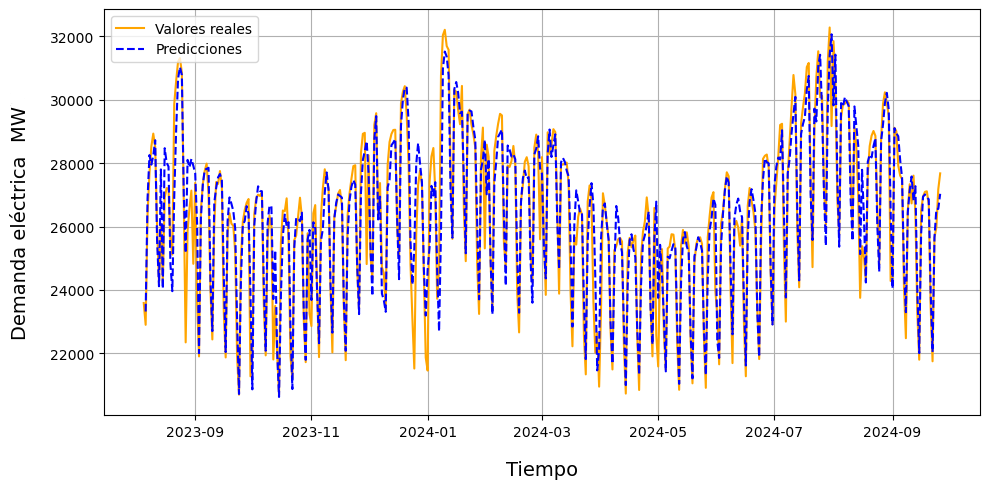
\includegraphics[width=0.9\textwidth]{Images/tfm-4.3(randomforest).png}
    \caption{Representación gráfica de los mejores resultados del modelo Random Forest (Elaboración propia) }
    \label{fig:figura_RM}
\end{figure}

La serie temporal del modelo con mejores resultados, correspondiente al Grupo 5 de variables exógenas, se puede observar en la Figura \ref{fig:figura_RM}. En general, el modelo se ha adaptado bastante bien a los datos de entrenamiento, exceptuando tres días festivos donde ha habido un mayor desacierto en la predicción: el día de la Asunción de la Virgen (18 de agosto), el día de Navidad (25 de diciembre) y el día de Año Nuevo (1 de enero). Aparte de estos días puntuales, las predicciones han sido más acertadas, captando mejor los patrones de baja demanda semanales, aunque se ha mantenido un pequeño error apreciable.

\subsection{Modelo XGBoost}

\begin{table}[H]
\centering
\caption{\\ Resultados de la optimización del modelo XGBoost}
\scriptsize
\begin{tabular}{m{1cm} m{1.2cm} m{1.2cm} m{1cm} m{1cm} m{1.2cm} m{1.2cm} m{3.5cm}} 
\toprule
\textbf{Modelo} & \textbf{V. exóg.} & \textbf{Optim.} & \textbf{t (s)} & \textbf{it} & \textbf{t/it (s)} & \textbf{MAE} & \textbf{Hiperparámetros} \\
\midrule
XGBoost   & Grupo 0 & Bayesiana & 504,87 & 200 & 2,52 & 843,94 & \texttt{$n\_estimators=330$ \newline $max\_depth=6$ \newline $learning\_rate=0,02$ \newline $subsample=0,63$ \newline $colsample\_bytree=0,94$ \newline $gamma=0,87$ \newline $reg\_alpha=0,998$ \newline $reg\_lambda=0,77$} \\[0.5em]
\hline
XGBoost   & Grupo 1 & Bayesiana & 518,32 & 200 & 2,59 & 709,73 & \texttt{$n\_estimators=220$ \newline $max\_depth=8$ \newline $learning\_rate=0,02$ \newline $subsample=0,27$ \newline $colsample\_bytree=0,98$ \newline $gamma=0,97$ \newline $reg\_alpha=0,81$ \newline $reg\_lambda=0,63$} \\[0.5em]
\hline
XGBoost   & Grupo 2 & Bayesiana & 478,78 & 200 & 2,39 & 697,02 & \texttt{$n\_estimators=280$ \newline $max\_depth=4$ \newline $learning\_rate=0,03$ \newline $subsample=0,53$ \newline $colsample\_bytree=0,80$ \newline $gamma=0,56$ \newline $reg\_alpha=0,97$ \newline $reg\_lambda=0,79$} \\[0.5em]
\hline
XGBoost   & Grupo 3 & Bayesiana & 482,05 & 200 & 2,41 & 625,15 & \texttt{$n\_estimators=260$ \newline $max\_depth=3$ \newline $learning\_rate=0,06$ \newline $subsample=0,38$ \newline $colsample\_bytree=0,99$ \newline $gamma=0,80$ \newline $reg\_alpha=0,92$ \newline $reg\_lambda=0,90$} \\[0.5em]
\hline
XGBoost   & Grupo 4 & Bayesiana & 499,94 & 200 & 2,50 & 579,05 & \texttt{$n\_estimators=240$ \newline $max\_depth=3$ \newline $learning\_rate=0,04$ \newline $subsample=0,60$ \newline $colsample\_bytree=0,93$ \newline $gamma=0,60$ \newline $reg\_alpha=0,97$ \newline $reg\_lambda=0,83$} \\[0.5em]
\hline
XGBoost   & Grupo 5 & Bayesiana & 522,05 & 200 & 2,61 & 575,79 & \texttt{$n\_estimators=230$ \newline $max\_depth=3$ \newline $learning\_rate=0,08$ \newline $subsample=0,53$ \newline $colsample\_bytree=0,77$ \newline $gamma=0,86$ \newline $reg\_alpha=0,42$ \newline $reg\_lambda=0,24$} \\
\bottomrule
\end{tabular}
\label{tab:resultados_optimizacion_xgboost}
\caption*{\textit{Nota}: los hiperparámetros son \textit{n\_estimators}: number of estimators; \textit{max\_depth}: maximum depht ; \textit{learning\_rate}: learning rate; \textit{subsample}: subsample ratio of the training instances; \textit{colsample\_bytree}: subsample ratio of columns when constructing each tree; \textit{gamma}: gamma; \textit{reg\_alpha}: alpha; \textit{reg\_lambda}: lambda. (Elaboración propia)}
\end{table}

Como en los dos casos anteriores, se ha fijado el número de iteraciones en 200 y se ha utilizado la técnica de optimización bayesiana, acotando el espacio de hiperparámetros cada vez más a medida que se realizan más intentos.

La mejora entre el primer grupo de variables y el último ha sido bastante significativa, con una mejora aproximada del 32$\%$ en los resultados, considerando el MAE. A medida que se han ido añadiendo variables exógenas, los resultados han mejorado, siendo verdaderamente importantes las variaciones provocadas por las variables \textit{diasem}, \textit{festivo} y \textit{tmed}.

El valor de los hiperparámetros ha ido variando en cierta medida conforme se han entrenado los modelos con distintas variables exógenas. El hiperparámetro \textit{n\_estimators} ha fluctuado entre 220 y 330, alcanzando su punto más alto en el caso correspondiente al Grupo 0 de variables. Esto indica que la complejidad del modelo ha sido mayor en este caso, lo que ha llevado a una menor capacidad para captar los patrones en los datos. En general, las profundidades de los árboles han sido bajas, destacándose especialmente las de los tres últimos grupos de modelos. Por otro lado, el valor de \textit{learning\_rate} ha sido bastante bajo en todos los casos, observándose el mayor valor en el último modelo. Los parámetros \textit{subsample} y \textit{colsample\_bytree} reflejan cómo se muestrean los datos y las características. A medida que disminuyen sus valores, se utiliza una menor cantidad de datos para el entrenamiento. En estos casos, es mejor tener un valor equilibrado, al igual que para los hiperparámetros \textit{reg\_alpha} y \textit{reg\_lambda}, los cuales regulan el sobreajuste del modelo. Finalmente, \textit{gamma} se utiliza para controlar la complejidad del modelo; cuanto más alto es su valor, mayor es la penalización al crecimiento de los árboles.

En cuanto a los tiempos de procesamiento, el intervalo manejado en todos los casos se encuentra en torno a los 2-3 segundos por iteración. Esta escasa variabilidad sugiere que el modelo XGBoost se ha adaptado de manera satisfactoria a los datos de entrenamiento. El modelo que mejor combina complejidad y resultados es el correspondiente al Grupo 5 de variables exógenas.

\begin{figure}[H]
    \centering
    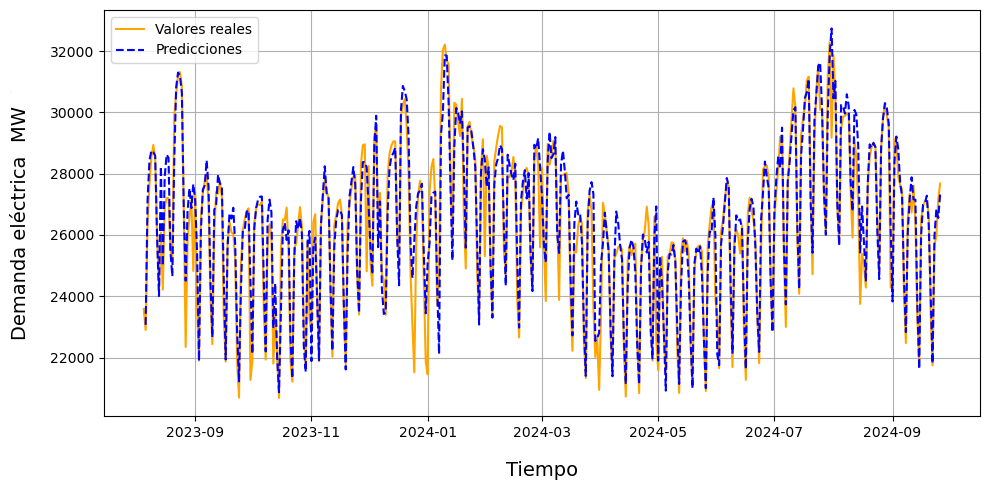
\includegraphics[width=0.9\textwidth]{Images/tfm-4.4(xgboost).png}
    \caption{Representación gráfica de los mejores resultados del modelo XGBoost (Elaboración propia) }
    \label{fig:figura_XG}
\end{figure}

La Figura \ref{fig:figura_XG} representa los mejores resultados obtenidos con el modelo XGBoost, correspondientes al Grupo 5 de variables exógenas. El modelo se ha adaptado de manera satisfactoria a los datos de entrenamiento, excepto en los días festivos, al igual que en el caso del Random Forest. A pesar de estos aspectos negativos, se observa que los resultados de la predicción son bastante realistas, captando adecuadamente la mayoría de los picos de demanda correspondientes a patrones semanales.

\subsection{Modelo LSTM}

\begin{table}[H]
\centering
\caption{\\ Resultados de la optimización del modelo LSTM}
\scriptsize
\begin{tabular}{m{1cm} m{1.2cm} m{1.2cm} m{1cm} m{1cm} m{1.2cm} m{1.2cm} m{3.5cm}} 
\toprule
\textbf{Modelo} & \textbf{V. exóg.} & \textbf{Optim.} & \textbf{t (s)} & \textbf{it} & \textbf{t/it (s)} & \textbf{MAE} & \textbf{Hiperparámetros} \\
\midrule
LSTM   & Grupo 0 & Grid Search & 1260,49 & 24 & 52,52 & 803,7 & \texttt{$recurrent\_units=110$ \newline $dense\_units=100$ \newline $learning\_rate=0,011$ \newline $epochs=45$} \\[0.5em]
\hline
LSTM   & Grupo 1 & Grid Search & 1273,18 & 24 & 53,05 & 686,24 & \texttt{$recurrent\_units=100$ \newline $dense\_units=110$ \newline $learning\_rate=0,011$ \newline $epochs=45$} \\[0.5em]
\hline
LSTM   & Grupo 2 & Grid Search & 1321,41 & 24 & 55,06 & 702,89 & \texttt{$recurrent\_units=100$ \newline $dense\_units=110$ \newline $learning\_rate=0,011$ \newline $epochs=40$} \\[0.5em]
\hline
LSTM   & Grupo 3 & Grid Search & 1326,55 & 24 & 55,27 & 695,26 & \texttt{$recurrent\_units=110$ \newline $dense\_units=100$ \newline $learning\_rate=0,011$ \newline $epochs=45$} \\[0.5em]
\hline
LSTM   & Grupo 4 & Grid Search & 1331,28 & 24 & 55,47 & 673,04 & \texttt{$recurrent\_units=100$ \newline $dense\_units=90$ \newline $learning\_rate=0,0115$ \newline $epochs=45$} \\[0.5em]
\hline
LSTM   & Grupo 5 & Grid Search & 1347,9 & 24 & 56,16 & 628,92 & \texttt{$recurrent\_units=110$ \newline $dense\_units=110$ \newline $learning\_rate=0,011$ \newline $epochs=45$} \\
\bottomrule
\end{tabular}
\label{tab:resultados_optimizacion_lstm}
\caption*{\textit{Nota}: los hiperparámetros son \textit{recurrent\_units}: recurrent units; \textit{dense\_units}: dense units ; \textit{learning\_rate}: learning rate; \textit{epochs}: number of epochs. (Elaboración propia)}
\end{table}

Para la optimización de los modelos, se ha utilizado la técnica de Grid Search en un espacio de hiperparámetros reducido, con un total de 24 iteraciones. Se realizaron entrenamientos previos que permitieron identificar una buena combinación de hiperparámetros para optimizar. No todos los hiperparámetros fueron explorados, ya que el \textit{batch size} ha sido fijado a 8 y para el \textit{optimization algorithm} solo se ha usado la función Adam.

Para controlar el sobreajuste de los modelos en cada uno de los grupos de variables exógenas, se realiza un análisis de la pérdida de entrenamiento y validación en función del número de épocas. En la Figura \ref{fig:figura_EVSV} se muestra la representación gráfica de cada uno de los modelos. En general, se observa que ambas curvas son bastante cercanas y casi paralelas en la mayoría de las épocas, con algunas variaciones leves. Además, ambas curvas descienden de forma similar, lo cual indica que se ha logrado controlar adecuadamente la generalización del modelo y, en consecuencia, el sobreajuste.

\begin{figure}[H]
    \centering
    % Primera columna de imágenes (3 filas)
    \begin{subfigure}{0.45\textwidth}
        \centering
        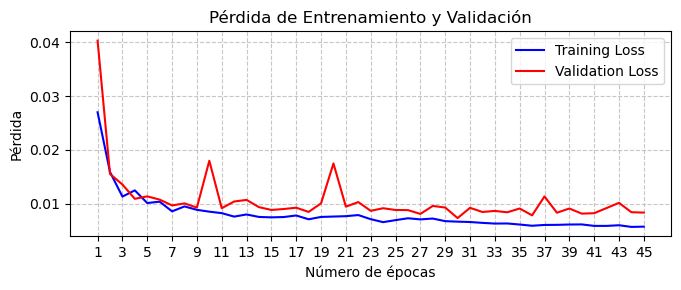
\includegraphics[width=\textwidth]{Images/tfm-4.6.0.png}
        \caption{Grupo 0}
    \end{subfigure}
    \begin{subfigure}{0.45\textwidth}
        \centering
        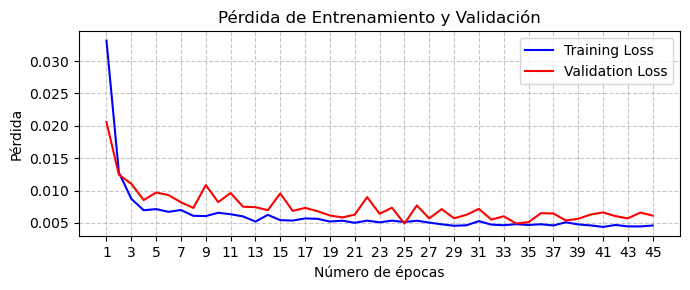
\includegraphics[width=\textwidth]{Images/tfm-4.6.1.png}
        \caption{Grupo 1}
    \end{subfigure}
    
    % Segunda fila de imágenes
    \begin{subfigure}{0.45\textwidth}
        \centering
        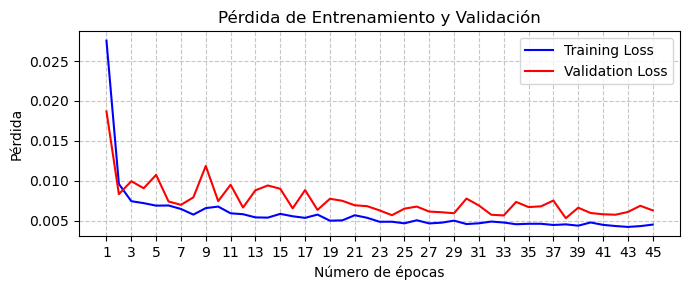
\includegraphics[width=\textwidth]{Images/tfm-4.6.2.png}
        \caption{Grupo 2}
    \end{subfigure}
    \begin{subfigure}{0.45\textwidth}
        \centering
        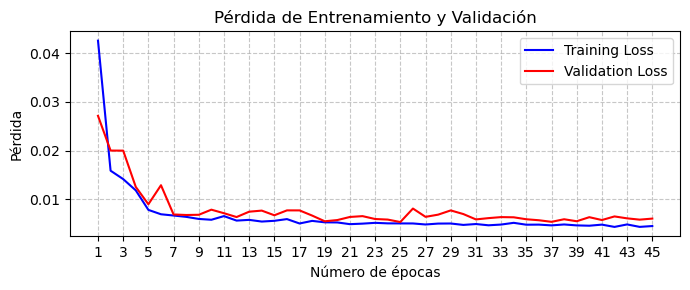
\includegraphics[width=\textwidth]{Images/tfm-4.6.3.png}
        \caption{Grupo 3}
    \end{subfigure}
    
    % Tercera fila de imágenes
    \begin{subfigure}{0.45\textwidth}
        \centering
        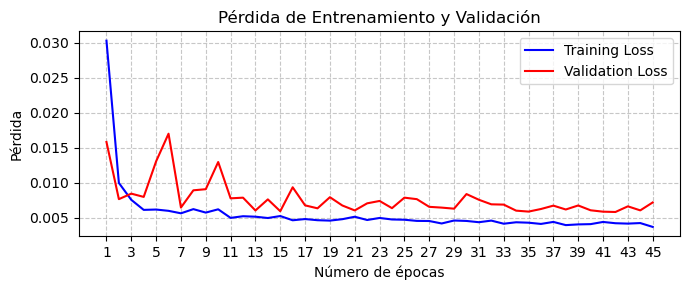
\includegraphics[width=\textwidth]{Images/tfm-4.6.4.png}
        \caption{Grupo 4}
    \end{subfigure}
    \begin{subfigure}{0.45\textwidth}
        \centering
        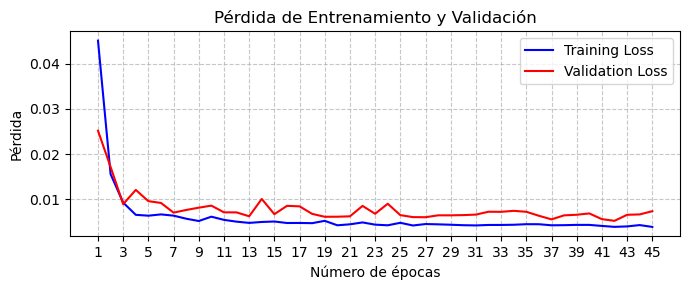
\includegraphics[width=\textwidth]{Images/tfm-4.6.5.png}
        \caption{Grupo 5}
    \end{subfigure}
    \caption{Pérdida de entrenamiento y validación para cada grupo de variables exógenas (Elaboración propia)}
    \label{fig:figura_EVSV}
\end{figure}

En aspectos generales, se puede observar que el MAE se ha ido reduciendo de manera prograsiva según se han añadido variables exógenas, exceptuando el caso del Grupo 2, donde el modelo ha empeorado los resultados anteriores al añadir la variable \textit{trim}. Además, la adición de la variable \textit{festivo}, no ha mejorado prácticamente la calidad de los resultados. Se ha observado que conforme aumentaba el número de \textit{recurrent\_units} y \textit{dense\_units} el MAE iba reduciéndose, coincidiendo con la incorporación de nuevas variables exógenas. El hiperparámetro \textit{epochs} no ha seguido un patrón claro, al igual que el \textit{learning\_rate}. La mejora del último grupo con respecto al primero ha sido del 21$\%$ aproximadamente.

Los tiempos de procesamiento han sido bastantes altos en todas las iteraciones, y siendo levemente superiores conforme se añaden variables exógenas. Siempre se han movido en el intervalo de 52 a 57 segundos por iteración.



\begin{figure}[H]
    \centering
    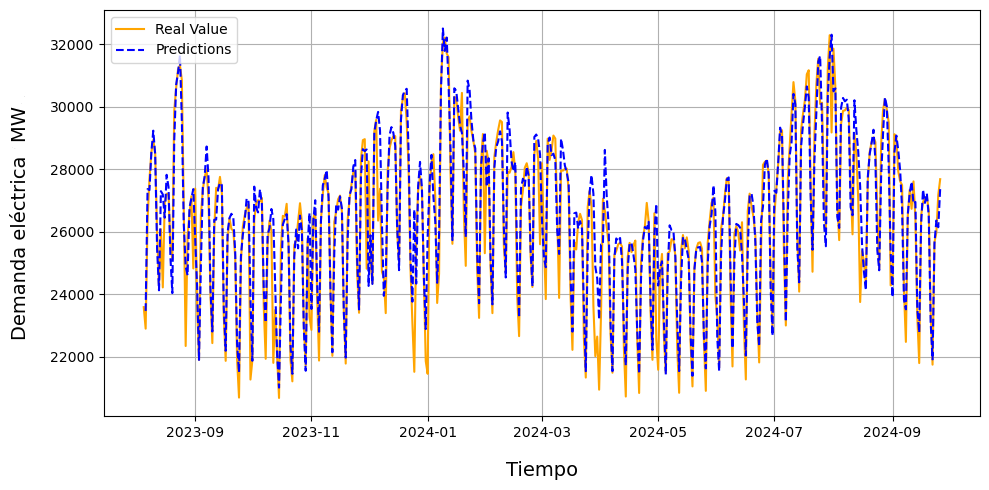
\includegraphics[width=0.9\textwidth]{Images/tfm-4.5(lstm).png}
    \caption{Representación gráfica de los mejores resultados del modelo LSTM (Elaboración propia) }
    \label{fig:figura_LSTM}
\end{figure}


La figura \ref{fig:figura_LSTM} muestra los resultados correspondientes al mejor MAE para el Grupo 5 de variables exógenas. Se observa que los picos de baja demanda semanales se han estimado con ciertos márgenes de error que se han mantenido prácticamente uniformes en la serie. Hay algunas excepciones donde el modelo no ha capturado los patrones de manera adecuada, principalmente en algunos días festivos. El resto de los patrones sí han sido estimados de manera satisfactoria.









\section{Comparativa general de los resultados}

Una vez analizados los resultados de cada conjunto de grupos de variables exógenas de los modelos individuales, se deben examinar y comparar los resultados de todos los modelos de manera general. Para ello, se han extraído los mejores resultados de cada modelo y se presentan en la Tabla \ref{tab:resultados_generales}.

\begin{table}[H]
\centering
\caption{\\ Mejor resultado de cada modelo}
\scriptsize
\begin{tabular}{m{1cm} m{1.2cm} m{1.2cm} m{1cm} m{1cm} m{1.2cm} m{1.2cm} m{3.5cm}} 
\toprule
\textbf{Modelo} & \textbf{V. exóg.} & \textbf{Optim.} & \textbf{t (s)} & \textbf{it} & \textbf{t/it (s)} & \textbf{MAE} & \textbf{Hiperparámetros} \\
\midrule
ARIMAX  & Grupo 5 & Grid Search & 438,50 & 27 & 16,24 & 772,99 & \texttt{$p=2$ \newline $d=1$ \newline $q=3$} \\
\hline
Decision Tree   & Grupo 4 & Bayesiana & 154,40 & 200 & 0,90 & 790,53 & \texttt{$max\_depth=11$ \newline $max\_leaf\_nodes=53$ \newline $min\_samples\_leaf=4$ \newline $min\_samples\_split=17$} \\[0.5em]
\hline
Random Forest   & Grupo 5 & Bayesiana & 660,65  & 200 & 3,30 & 641,08 & \texttt{$n\_estimators=130$ \newline $max\_depth=18$ \newline $max\_leaf\_nodes=67$ \newline $min\_samples\_leaf=2$ \newline $min\_samples\_split=19$ \newline $max\_samples=0,64$} \\
\hline
XGBoost   & Grupo 5 & Bayesiana & 522,05 & 200 & 2,61 & 575,79 & \texttt{$n\_estimators=230$ \newline $max\_depth=3$ \newline $learning\_rate=0,08$ \newline $subsample=0,53$ \newline $colsample\_bytree=0,77$ \newline $gamma=0,86$ \newline $reg\_alpha=0,42$ \newline $reg\_lambda=0,24$} \\
\hline
LSTM   & Grupo 5 & Grid Search & 1347,9 & 24 & 56,16 & 628,92 & \texttt{$recurrent\_units=110$ \newline $dense\_units=110$ \newline $learning\_rate=0,011$ \newline $epochs=45$} \\
\bottomrule
\end{tabular}
\label{tab:resultados_generales}
\caption*{\textit{Nota}: (Elaboración propia)}
\end{table}

En general, se observa que los modelos pertenecientes a la familia de los árboles han logrado el mejor equilibrio entre resultados y rendimiento, todos ellos optimizados mediante técnicas bayesianas. Aunque el modelo Decision Tree ha presentado el peor valor en el MAE de todos los modelos, ha demostrado ser la técnica con mayor rendimiento, con un tiempo por iteración de menos de un segundo. Random Forest ha mejorado los resultados en comparación con el modelo anterior, pero ha incrementado el tiempo de procesamiento, aunque mantiene tiempos relativamente bajos. Sin embargo, el modelo que ha obtenido un rendimiento más que aceptable y los mejores resultados entre todos los modelos ha sido XGBoost. Esta técnica ha mostrado una capacidad notable para captar los patrones subyacentes en los datos, a pesar de no haber podido predecir algunos días con picos de demanda bastante bajos, como es el caso de algunos días festivos.

En cuanto al resto de los modelos, ARIMAX ha obtenido resultados levemente superiores a los del modelo Decision Tree, pero con un tiempo de procesamiento unas 18 veces mayor. Este modelo ha establecido pautas en relación con los resultados tanto predictivos como de procesamiento. Se ha observado que ARIMAX puede funcionar satisfactoriamente cuando los patrones en los datos son relativamente sencillos; sin embargo, cuando se enfrentan a problemas más complejos que incluyen relaciones no lineales, presenta mayores limitaciones en sus habilidades predictivas.

En cuanto al modelo de Deep Learning estudiado, LSTM, no se han obtenido los mejores resultados en comparación con los pronósticos iniciales. Debido a la mayor complejidad del modelo en relación con los demás, la optimización de los hiperparámetros ha sido más tediosa, ya que no se han empleado técnicas más avanzadas y se ha optado por un simple Grid Search. Además, la cantidad limitada de datos y la poca complejidad de la estructura de la red neuronal elegida posiblemente no han permitido extraer el verdadero potencial del modelo. A pesar de esto, los resultados han sido bastante satisfactorios, situándose solo por detrás del modelo XGBoost. Cabe destacar que el procesamiento ha sido considerablemente costoso, un hecho que era de esperar debido a la complejidad computacional que acarrean este tipo de algoritmos, superando los tiempos de cada iteración en casi 22 veces respecto al modelo que ha obtenido los mejores resultados, XGBoost.

Sin ninguna duda, el modelo que mejor se ha adaptado a los patrones de los datos suministrados ha sido XGBoost, obteniendo los mejores resultados en la métrica del MAE y con costos computacionales más bajos, solo superado por el modelo Decision Tree. Además, debido a la estabilidad observada en la optimización de sus hiperparámetros y a la calidad de los resultados, ha sido el modelo que mejor se ha generalizado.

Paralelamente, se ha podido comprobar que, en la mayoría de los casos, la adición de variables exógenas ha mejorado los resultados predictivos, excepto en ocasiones puntuales en las que el modelo en cuestión no ha sido capaz de capturar las nuevas relaciones. A pesar de ello, se ha observado que dos variables exógenas no han aportado información de calidad e incluso han introducido ruido en algunas ocasiones. Estas variables son \textit{trim} y \textit{hrmed}, destacando principalmente la primera. Sería necesario considerar si realmente estas variables tienen una relación lo suficientemente significativa con la variable objetivo, o si existe cierta dependencia con otras variables exógenas que esté redundando en la información y ocasionando ruido.

\chapter{Conclusiones y trabajos futuros}\label{cap:cap4}

Los resultados expuestos en la sección anterior permiten comparar los objetivos iniciales propuestos en el proyecto con los logros alcanzados. De esta manera, se pueden extraer conclusiones que aporten valor al desarrollo del trabajo, destacando tanto los aspectos positivos como los aspectos por mejorar. Esto abre la puerta a optimizar la metodología y los procesos técnicos implementados e, incluso, a expandir el desarrollo hacia otras áreas.

\section{Conclusiones}

Tal y como se ha mencionado, para poder hacer unas conclusiones adecuadas del proyecto, se debe de hacer una comparación con los objetivos propuestos al inicio, tanto principales como secundarios. 

Siguiendo el desarrollo del proyecto, se observa que la extracción de datos se realizó a partir de fuentes oficiales, como AEMET y REE, lo cual garantiza la fiabilidad, coherencia e integridad de los datos utilizados. El proyecto se concibió para comparar el desempeño de algoritmos con distintas características en la predicción de la demanda eléctrica, por lo que se optó por utilizar datos con frecuencia diaria en lugar de horaria, permitiendo un análisis más amplio en un periodo más corto. Esta decisión ha tenido un impacto significativo en el desempeño de los modelos, especialmente en el caso del modelo LSTM.

El entrenamiento de los cinco modelos distintos ha requerido un estudio exhaustivo del marco teórico, permitiendo profundizar en el funcionamiento de cada uno. Esto ha facilitado una optimización de hiperparámetros de calidad, evitando el sobreajuste y promoviendo una buena generalización de los resultados. Cabe señalar que los largos tiempos de procesamiento, especialmente en el caso del modelo LSTM, han dificultado la búsqueda óptima de hiperparámetros; sin embargo, esta problemática se ha mitigado gracias al seguimiento de la planificación previa de tareas.

En relación con el objetivo principal de analizar y comparar diferentes modelos de Machine Learning para el forecasting de la demanda eléctrica, los resultados obtenidos han mostrado buena precisión, aunque aún existe margen de mejora. El modelo que mejor se ha adaptado ha sido XGBoost, que presenta bajos costos de procesamiento y genera predicciones bastante precisas. Sin embargo, ha mostrado dificultades para captar los picos de baja demanda en patrones estacionales a nivel semanal y en días festivos. En segundo lugar, se encuentra el modelo de Deep Learning LSTM, lo cual ha desafiado la hipótesis inicial del proyecto, que preveía que este modelo ofrecería el mejor desempeño. Contrario a las expectativas, LSTM ha requerido tiempos de procesamiento significativamente más largos, y aunque no se descarta su potencial, los resultados sugieren que un conjunto de datos de mayor granularidad, por ejemplo, a nivel horario, podría mejorar su precisión. En el contexto de este proyecto, con la cantidad de datos y variables seleccionadas, se puede afirmar con certeza que el mejor desempeño lo ha obtenido el modelo XGBoost.

En cuanto a los factores que influyen en la demanda eléctrica, se puede afirmar que las variables exógenas seleccionadas han mostrado un buen desempeño, destacándose especialmente los días de la semana, los días festivos y la temperatura. En cambio, otras variables, como el trimestre y la humedad relativa, han tenido un impacto variable: en algunos casos han mejorado levemente los resultados, mientras que en otros han introducido ruido que ha disminuido la capacidad predictiva de los modelos Decision Tree y Random Forest.

El seguimiento de la planificación de tareas ha sido en general bastante fiel a lo propuesto inicialmente, salvo que las etapas iniciales requirieron menos tiempo del previsto, lo cual se compensó en semanas posteriores. En conjunto, este proyecto ha permitido aplicar una amplia variedad de conocimientos y habilidades adquiridas en el Máster, incluida la capacidad de autoaprendizaje. Esto ha facilitado un análisis propio de las fortalezas y debilidades del trabajo. Aunque los resultados obtenidos son satisfactorios, existe un margen de mejora que podría explorarse en futuros estudios.

\section{Trabajos futuros}

Las limitaciones de este proyecto abren oportunidades para trabajos futuros, tanto en el ámbito de la predicción de demanda eléctrica como en otros campos de la ciencia de datos, especialmente en forecasting. Una posible línea de mejora sería ampliar el conjunto de variables exógenas, integrando otras variables meteorológicas, indicadores económicos o factores no considerados en este estudio. También se podría investigar cómo variarían los resultados de los modelos si se entrenaran con un conjunto de datos más amplio, de frecuencia horaria en lugar de diaria. Dado el potencial del modelo LSTM, sería interesante explorar algoritmos de optimización más avanzados, como el descenso de gradiente. En general, los conocimientos adquiridos en este proyecto pueden aplicarse a otros campos basados en forecasting, como otras ramas de la energía, el sector bancario y el mundo del comercio.

\appendix
\printbibliography
\addcontentsline{toc}{chapter}{Referencias} 


\end{document}
